\chapter{流量异常检测系统的设计与实现}
\section{引言}
本章结合前四章的分析和结论,将基于特征关系图的RNN模型应用到实际流量环境中,验证其真实有效性。因此本文针对清华大学校园网的流量环境,设计了一个流量异常检测系统。该系统应该满足以下几点要求:
\begin{enumerate}
  \item 实时性。如果一个系统检测延迟很高,那么即使其准确率同样很高,这个检测结果也将毫无意义。因为异常检测的目的是在攻击的早期阶段就将其发现,并且作出应对。
  \item 高效性。校园网用户规模大,流量峰值高,该系统需要能够高效处理海量的流量数据。
  \item 鲁棒性。该系统应该保证能够在复杂的网络环境面前依然有较好的检测效果,例如发生突出事件或者新的异常类型时依然能够有一定的检测效果。
  \item 模块化。该系统的各个模块之间的耦合度应尽可能低,一方面便于调试,另一方面可以便捷的验证其他算法模型。
\end{enumerate}

本文的流量异常检测系统按照上述需求设计如图\ref{fig:arch}所示,可以分为三个模块:输入模块、检测模块、输出模块。其中输入模块将流量数据和SOC标签数据整合成特征数据;模型模块分为离线训练和在线检测两部分,离线训练部分定期产出更新好参数的模型,在线检测部分会接受当前的特征数据进行判别;最后输出模块将判别结果并根据历史信息进行异常等级划分,给运维人员下一步提供参考。
% TODO: 图中加入关系矩阵
\begin{figure}
    \centering
    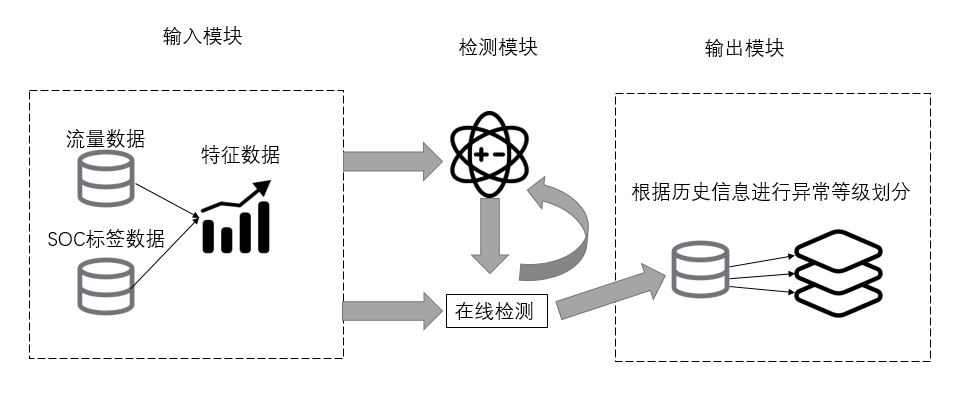
\includegraphics[scale=0.55]{系统架构图.png}
    \caption{系统架构图}
    \label{fig:arch}
  \end{figure}


\section{Spark 平台介绍}
Spark Streaming贯穿本节系统的始终,因此首先对Spark和Spark Streaming做一个简单介绍。

Apache Spark是由UC Berkeley AMP Lab开源的用于大规模数据处理的统一分析引擎\cite{spark},现如今已经成为Apache软件基金会的最为出名的开源项目之一。Spark原理与Hadoop类似,都是基于MapReduce进行分布式计算,但是功能更加丰富,且支持SQL查询、流式处理、图计算等功能。

Spark具有以下几个特点:

\begin{itemize}
  \item 速度快。这是因为Spark基于内存计算,而Hadoop MapReduce必须进行读取和写入磁盘,IO操作比内存操作更加耗时。图\ref{fig:Logistic regression in Hadoop and Spark}是Spark官网给出的一项逻辑回归任务在Hadoop和Spark两个系统的运行时长对比。
   \begin{figure}
    \centering
    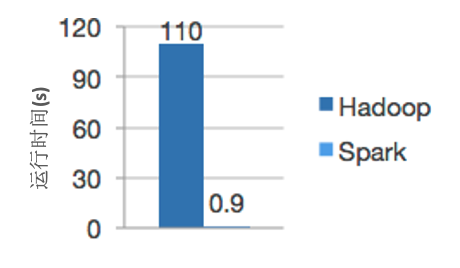
\includegraphics[width=0.3\linewidth]{logistic-regression.png}
    \caption{Logistic regression in Hadoop and Spark}
    \label{fig:Logistic regression in Hadoop and Spark}
  \end{figure}
  \item 易用性。Spark提供了80余种高级API,可以轻松编写高度并行的应用程序。Spark支持Java, Scala, Python, R, and SQL等多种编程语言。
  \item 兼容性。Spark支持多种数据源作为输入,例如本地文件系统、HDFS、HBase等,并且Spark支持多种运行模式,能够做到类似java的“一次编写,多处运行”。
\end{itemize}



如图\ref{fig:Spark组件}所示\cite{spark},Spark项目包含多个独立组件。其最核心的模块为深蓝色的Spark Core,其定义了核心API,如“弹性分布式数据集”,该模块也负责调度、监控计算集群中的计算任务,具有内存管理、故障恢复、与管理系统和存储系统交互等功能。为了满足分布式计算系统的可扩展性,Spark支持在各种集群管理器之上运行,例如图中灰色的模块Hadoop YARN,Apache Mesos以及浅蓝色的Spark系统中包含的“独立调度程序”(Standalone Scheduler)。在Spark Core之上,具有浅蓝色的四个组件:Spark SQL(处理结构化数据),Spark Streaming(实时处理海量数据),MLlib(运行机器学习模型),GraphX(提供图计算)。本文中的系统主要使用Spark Streaming组件。



\begin{figure}
  \centering
  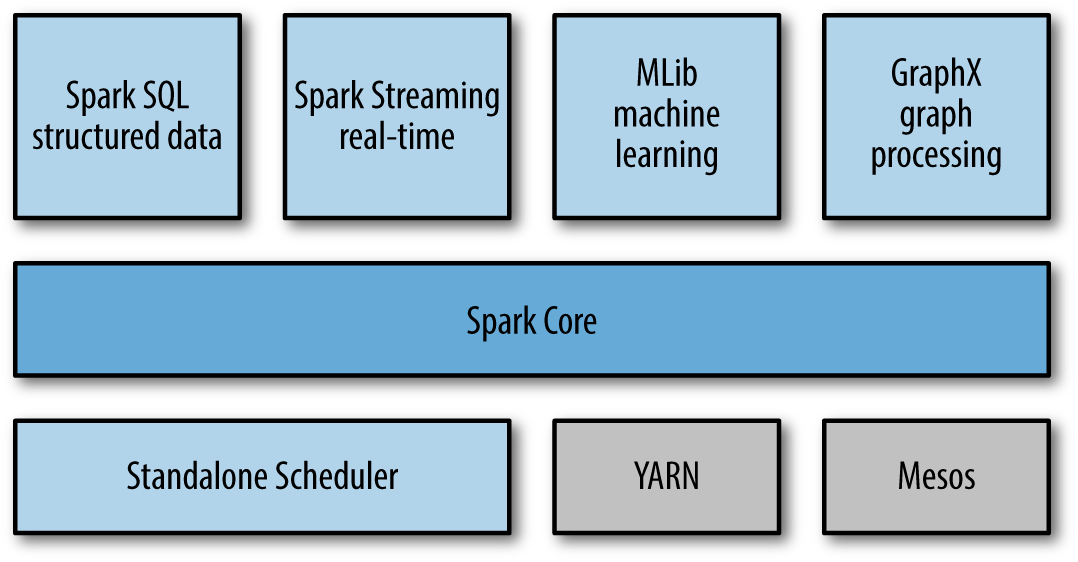
\includegraphics[width=0.6\linewidth]{spark-stack.png}
  \caption{Spark组件}
  \label{fig:Spark组件}
\end{figure}

图\ref{fig:spark工作原理}是Spark Streaming的基本工作原理\cite{spark}。Spark Streaming本质上是微批处理系统,其将输入数据流划分成批式数据,然后依次处理每批数据。
\begin{figure}
  \centering
  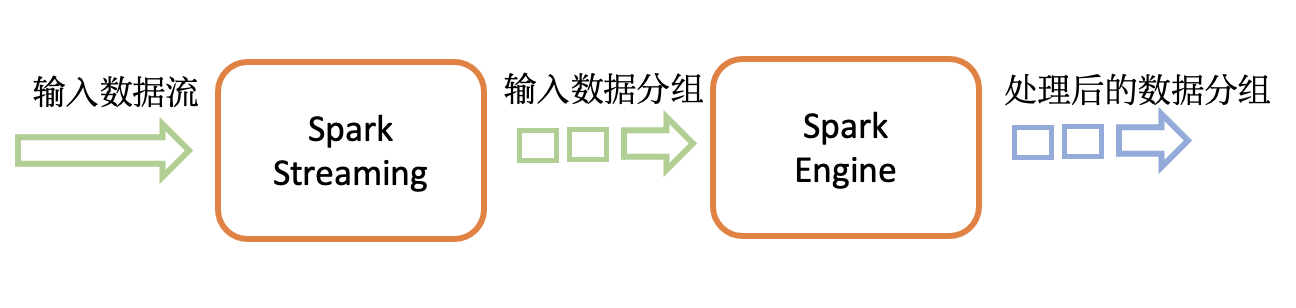
\includegraphics[scale=0.6]{spark工作原理.png}
  % 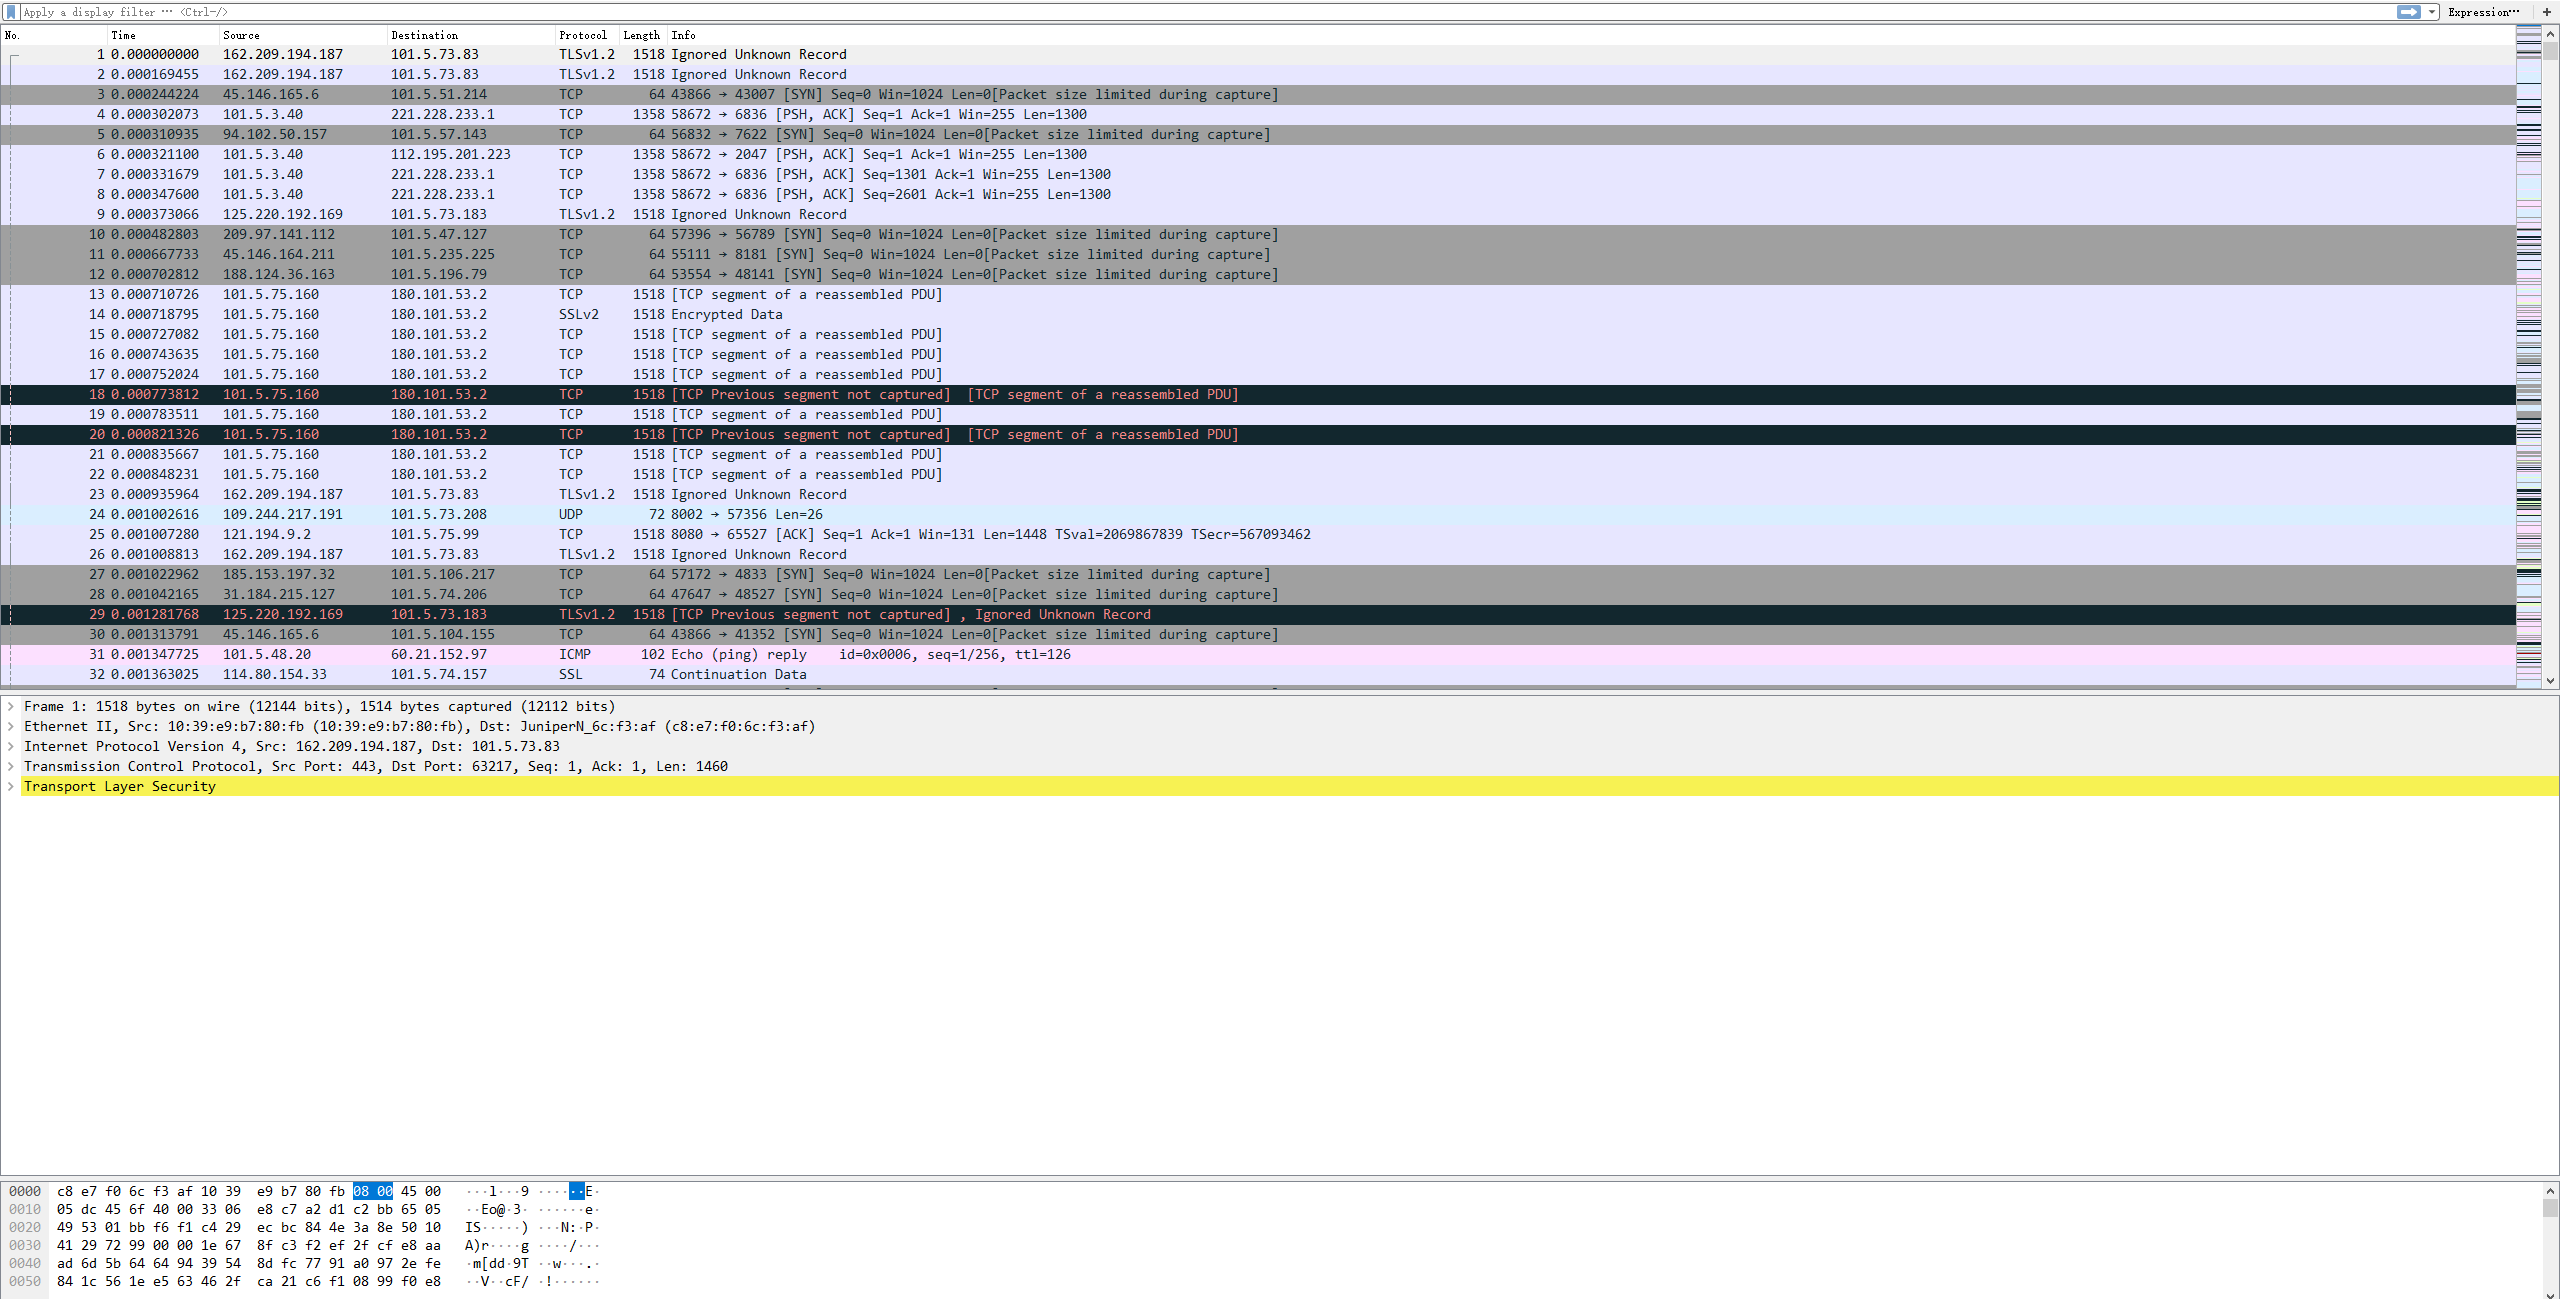
\includegraphics[width=0.6\linewidth]{wireshark流量图.png}
  \caption{Spark Streaming工作原理}
  \label{fig:spark工作原理}
\end{figure}

\section{系统各模块设计}
本文实现流量异常检测系统的架构如图\ref{fig:arch}所示,整个架构是基于Spark Streaming实现。本节将分模块具体介绍。
\subsection{输入模块}
输入模块的主要功能是对流式数据进行特征抽取,与第三章中的特征提取单一文件不同的是,本模块处理的数据是“无界”的。我们需要将无界数据进行切片,每次处理一个片段内的数据。这些片段又被称为“window”,window是流式计算领域的核心概念。

本模块的输入为由kafka传入的流量数据,然后将流量报文划分到一个个滑动窗口(sliding window)中,每次处理一个窗口内的全部报文。流量特征提取的整体流程图\ref{fig:特征提取}所示。读取到packet后,首先为每条报文建立一个由五元组信息组成的标志,然后根据图中的规则依次判断该报文是否是一条新的流的起始报文、是否是当前流的结束报文、是否需要调用updateflow更新各项统计信息。

\begin{figure}
  \centering
  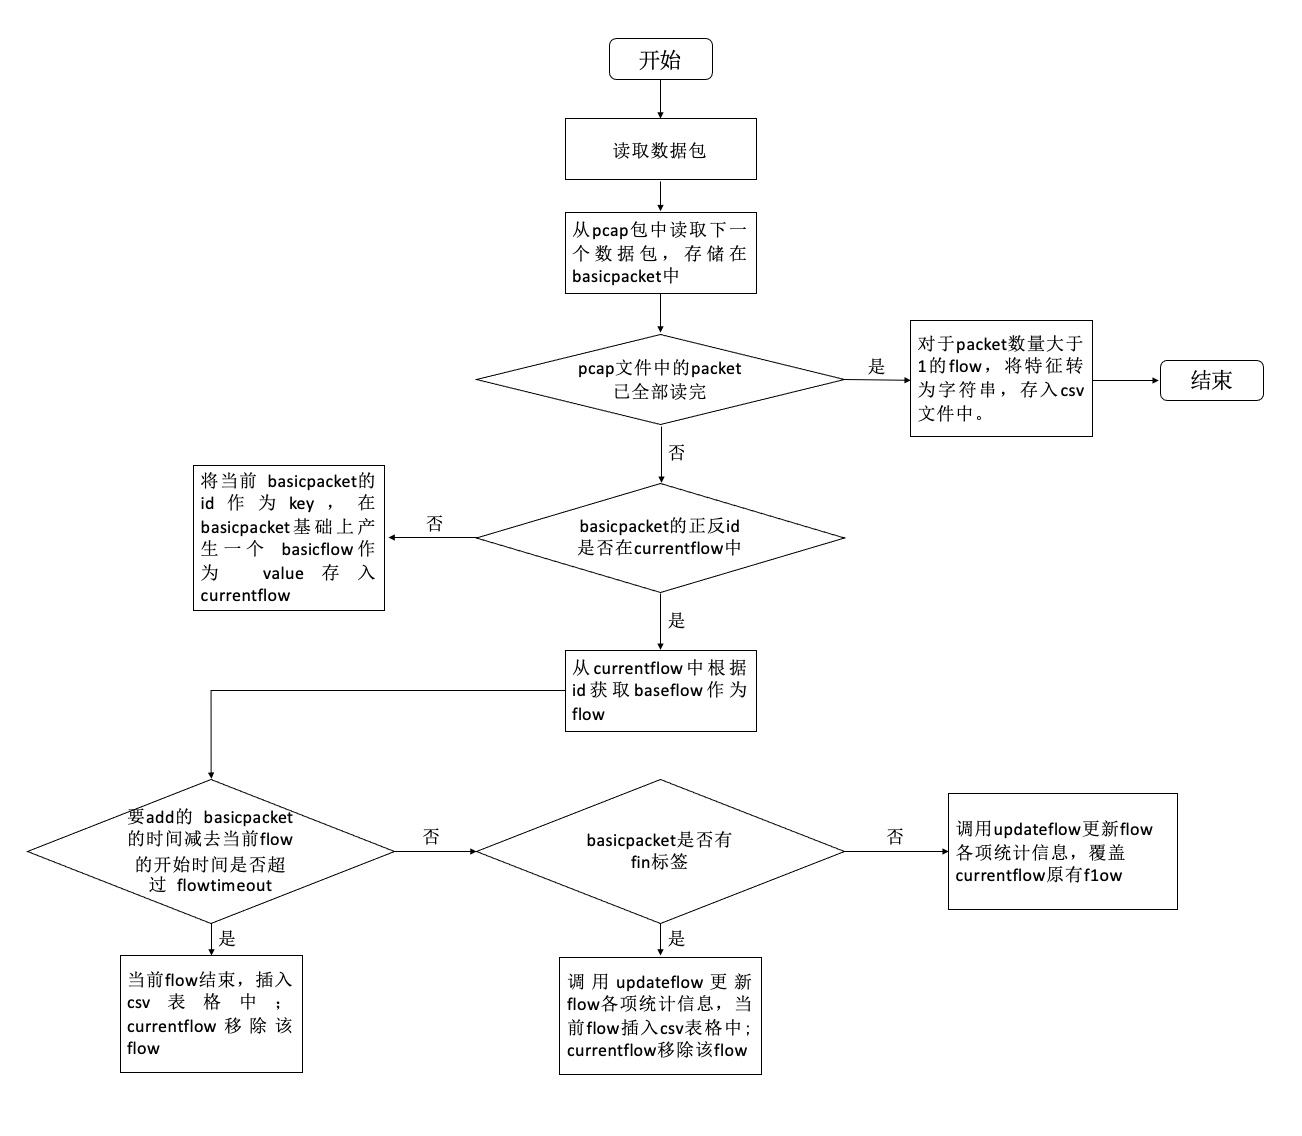
\includegraphics[scale=0.3]{特征提取.jpg}
  \caption{特征提取流程图}
  \label{fig:特征提取}
\end{figure}

本模块提取的结果是以一条TCP流或者UDP流为单位,该条流中全部报文的统计信息。在一条流中有很多个数据包,TCP流以三次握手为开始,以FIN标志为结束;UDP流以首次出现为开始,以超出超时时间为结束。并且每条流都是双向数据流,由源ip地址到目的ip地址为正向,目的ip地址到源ip地址为反向。

使用该方法得到的csv文件如图\ref{fig:特征文件}所示:
\begin{figure}
    \centering
    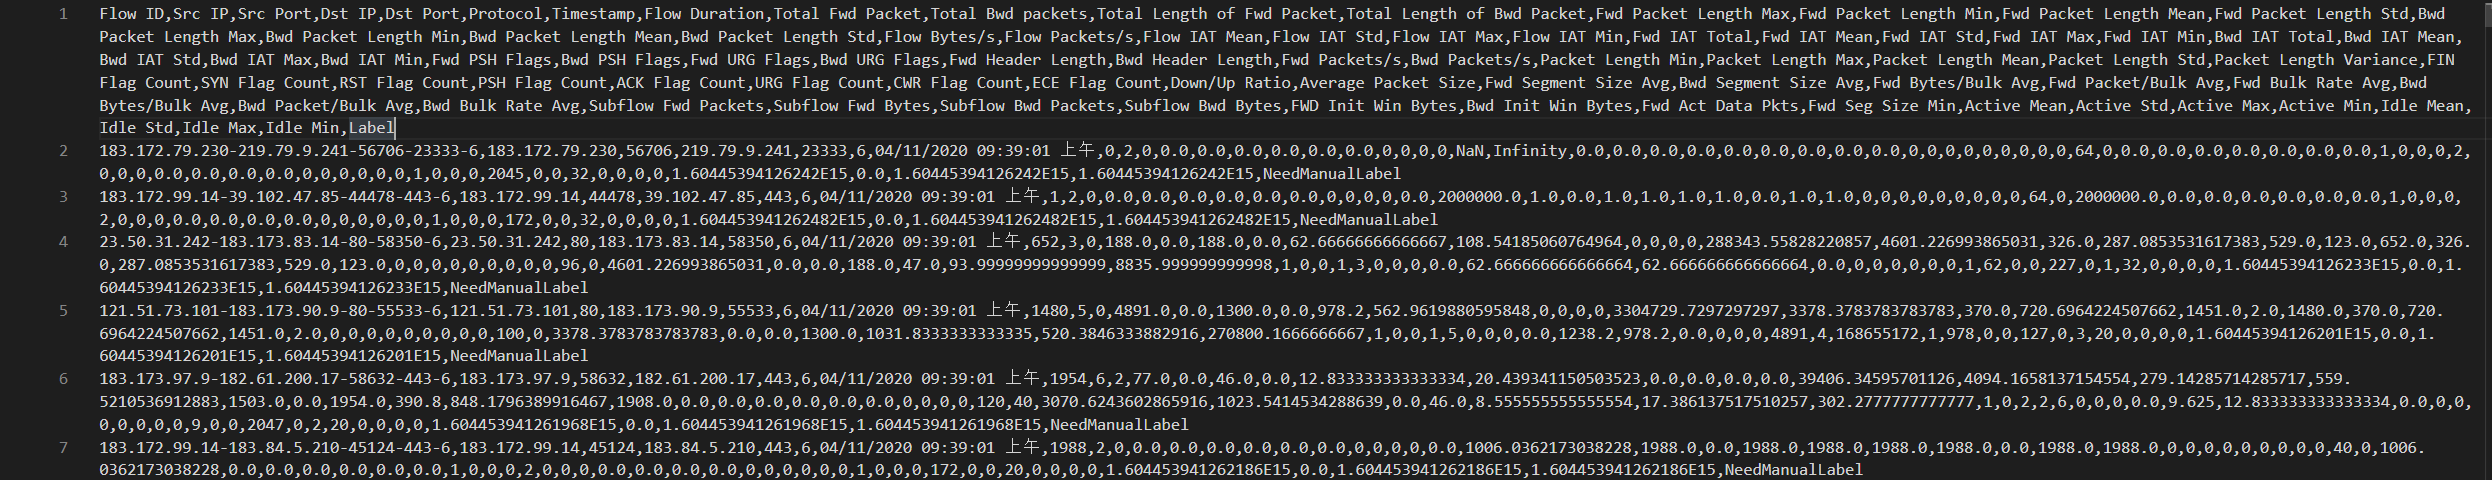
\includegraphics[scale=0.2]{特征文件.png}
    \caption{特征文件}
    \label{fig:特征文件}
  \end{figure}

% 得到特征文件后,需要进一步进行数据预处理。
% \begin{enumerate}
%   \item 删除无效信息,使用平均值填充空白值;
%   \item 对离散值进行one-hot编码,对连续值进行归一化;

% \end{enumerate}
\subsection{检测模块}
检测模块分为离线和在线两部分,并且由于第四章中FG-RNN算法的特点,特征关系图(Feature Graph)的更新频率与循环神经网络(RNN)不同,并且这两者在实现中已经解耦,因此RNN的参数更新仅需在离线部分完成,在线部分可以兼顾实时流量的检测和特征关系图参数的更新。该模块的架构图如图\ref{fig:检测模块架构图}所示。

\begin{figure}
  \centering
  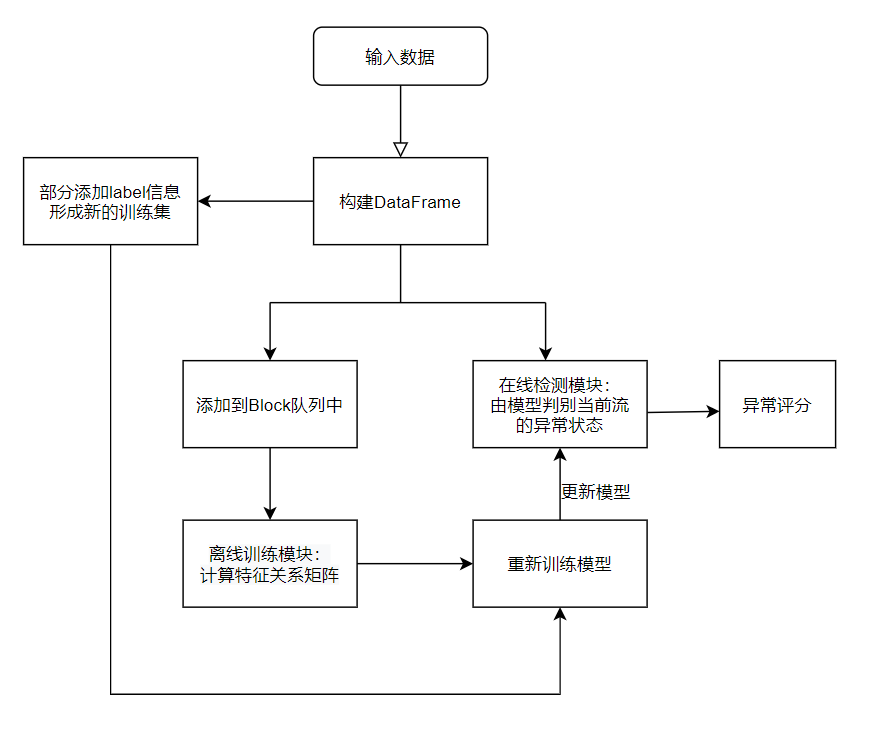
\includegraphics[scale=0.6]{检测模块架构图.png}
  \caption{检测模块架构图}
  \label{fig:检测模块架构图}
\end{figure}
该模块核心伪代码如下:
\begin{lstlisting}
  % 从kafka中读取DataFrame数据,转换成Spark Streaming的RDD
  kafkaStream = KafkaUtils.createDirectStream
      (ssc, dataframe, {"metadata.broker.list": brokers})

  % 离线训练,将RDD添加到block队列,计算特征关系矩阵
  kafkaStream.foreach(caculate_feature_graph)
  model = FGRNN(fg)
  model.save(sc, "path/models")
  
  % 在线检测,判别当前流的异常状态
  kafkaStream.foreach(model.predict)  
  \end{lstlisting}

该模块部分运行过程如图\ref{fig:检测模块运行过程}所示,

\begin{figure}
  \centering
  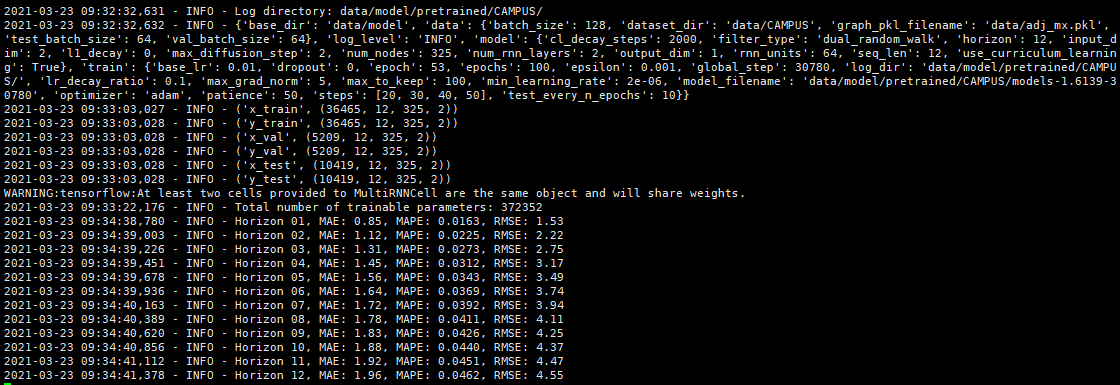
\includegraphics[scale=0.55]{检测运行过程.png}
  \caption{检测模块运行过程}
  \label{fig:检测模块运行过程}
\end{figure}

该模块实测运行过程中,我们发现模型检测效果会随时间剧烈衰减,如图\ref{fig:模型效果随时间衰减}所示,经过5小时后FG-RNN模型效果衰减到普通RNN模型的程度。本文中的模型本质上是一个时间序列模型,根据过去一段时间的数据的行为模式总结出历史规律然后对未来进行预测,将预测结果与真实数据对比达到检测异常的效果。因此模型准确率较高的一个前提是要预测的未来是训练数据集中历史规律的延续,测试集和训练集越相似,准确率就越高。但是在实际现网环境中,数据中的异常种类和数量在不断变化,时间间隔越大,数据集的行为模式差异越大。

% 由于数据集中异常种类多变,我们发现模型检测效果会随时间剧烈衰减,如图\ref{fig:模型效果随时间衰减}所示,经过5小时后FG-RNN模型效果衰减到普通RNN模型的程度,因此我们加入了动态更新特征图机制,实现模型稳定性。

而本文用来训练模型的数据集是一个静态数据集,只能描述过去一段时间的规律模式,随着时间变化,训练数据中的规律模式会逐渐不再准确,这必然导致模型在使用一段时间后会出现检测能力下降的现象,模型结果不可靠。

\begin{figure}
  \centering
  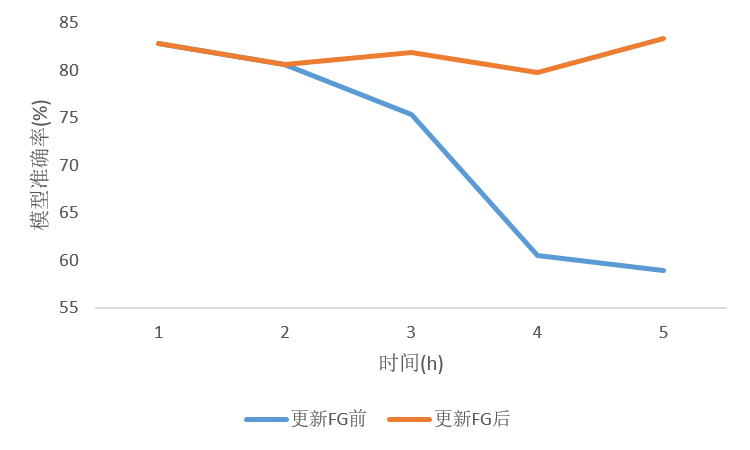
\includegraphics[scale=0.8]{模型效果随时间衰减.png}
  \caption{模型效果随时间衰减}
  \label{fig:模型效果随时间衰减}
\end{figure}

为了减缓模型检测效果衰减的速度,本文在系统中引入了动态更新特征图的机制,由于模型中的特征图代表了训练集的行为模式(pattern),本机制无需重新训练模型参数,仅通过更新特征图就可以满足需求。为了确定更新频率,我们计算了一段时间内的模型衰减程度,因为如果更新过快,则需要更多的算力,更新过慢,则检测效果不佳。如表\ref{模型衰减程度}所示,其中每段数据集时间间隔为半小时,最终我们设置2小时更新一次特征图。

\begin{table}[htb]
  \centering
  \caption{模型衰减程度}
  \label{模型衰减程度}
      \begin{tabular}{c|cccccccc}
      \toprule  % 在表格最上方绘制横线
      %  &数据集1 & 数据集2 &数据集3 & 数据集4 &数据集5 & 数据集6&数据集5 & 数据集6\\
      数据集序号&1 & 2 &3 & 4 &5 & 6&7 & 8\\
      \hline  %在第一行和第二行之间绘制横线
      模型准确率& 0.83 & 0.81& 0.79 & 0.78& 0.74 & 0.67& 0.63 & 0.61\\
      \hline % 在表格最下方绘制横线
      模型衰减程度& - & 0.02& 0.04 & 0.05& 0.09 & 0.16& 0.20 & 0.22\\
      \bottomrule % 在表格最下方绘制横线
      \end{tabular}
\end{table}


\subsection{输出模块}
在得到实时检测模块给出的异常流信息以及类型后,我们可以基于此做出进一步的处理。由于校园网流量“异常是常态,甚至半数流量是异常”的特点,若将全部异常信息都汇报给运维人员,大量危害程度低的异常告警势必会掩盖真正值得关注的异常,例如时刻都在发生的网络扫描,由于其重要性低微我们可以将其忽略。

因此,我们需要对异常的重要等级进行评分,具体的评分规则如下:首先初始化每种异常类型的基础分数,将异常分为低危、中危、高危三类,然后每次运维人员处理一条异常流后,将发现该流异常到处理异常的时间差作为权重,重新计算该异常的评分。



% \begin{figure}
%     \centering
%     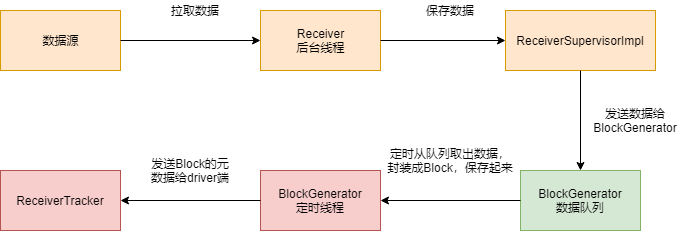
\includegraphics[scale=0.6]{spark数据源.png}
%     \caption{Spark数据源}
%     \label{fig:spark}
%   \end{figure}

% \section{流式数据特征抽取}
% Spark Streaming 支持 Scala、Java 和 Python,本文中使用Python提交任务。使用第三章中的特征提取方法,
% 输入为由kafka传入的流量数据,提取的结果都是传输层的一些统计信息,以一个TCP流或一个UDP流为一个单位。TCP流以FIN标志为结束,UDP以设置的flowtimeout时间为限制,超过时间就判为结束。在一个TCP流中有很多个数据包,先三次握手而后传输信息再四次挥手。统计一个流中的统计信息作为提取的特征。且统计的特征都分前后向,规定由源地址到目的地址为正向,目的地址到源地址为反向,例如某条TCP流的源ip地址为192.168.31.100,源端口号为174,目的ip地址为183.232.231.174,目的端口号为443,则为该流构建一个标志叫Flow ID:192.168.31.100-183.232.231.174-46927-443-6,由源地址、目的地址、源端口、目的端口、协议号组成。
% 流量特征提取的整体流程图如下:

% \begin{figure}
%     \centering
%     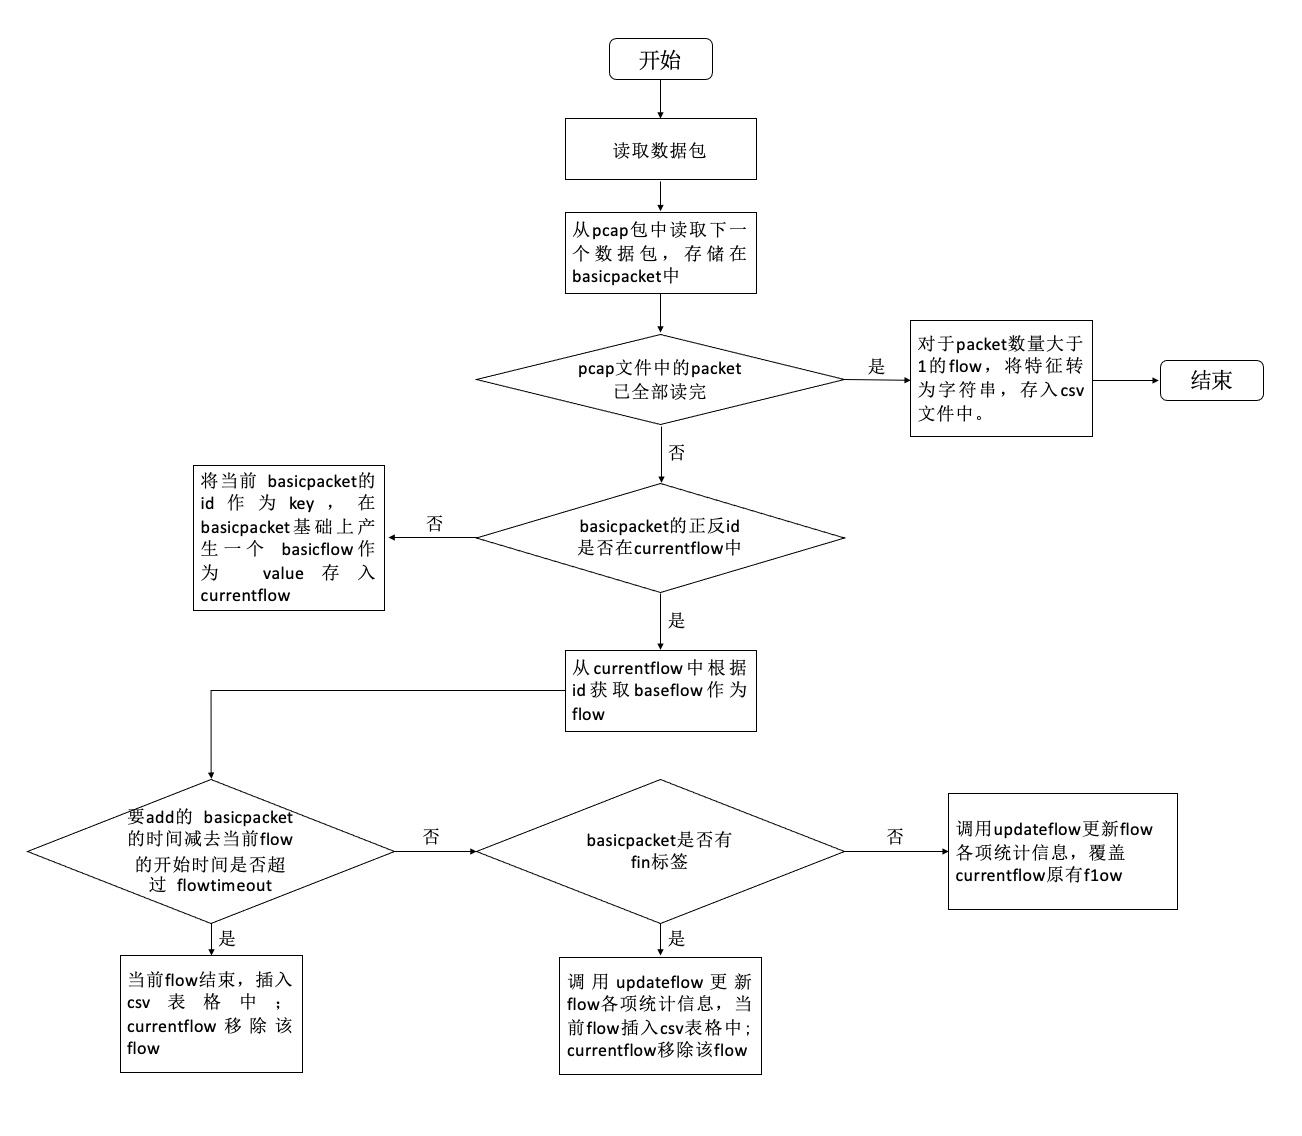
\includegraphics[scale=0.3]{特征提取.jpg}
%     \caption{特征提取}
%     \label{fig:特征提取}
%   \end{figure}


% 在currentFlows存储当前还未结束的所有TCP、UDP流。在添加的过程中不断地更新每个流的统计特征,最终将统计特征写入csv文件。判断新加入的数据包是否属于当前所有未结束的流,如果属于当前流则判断正向还是反向,之后判断时间是否超时、不超时则判断是否含有FIN标志,如果两者都不满足,则声明一个BasicFlow对象,根据id从currentFlows中拿到与当前数据包对应的流,调用addPacket将该数据包加入到对应流中。如果前面判断不在当前所有未结束的流中,则直接创建一个新的流,里面只含当前数据包,存入到currentFlows中。如果属于当前某个未结束的流,且超时或存在FIN标志,则说明当前flow结束,超时则从currentFlows中移除对应流,新建flow存入currentFlows中,含FIN标志则直接从currentFlows中移除对应流。结束的flow直接调用onFlowGenerated函数将流打印存储起来。




% \section{模型训练模块的设计与实现}
% 补充一些图
% \begin{figure}
%   \centering
%   
\includegraphics[width=0.6\linewidth]{example-image-a.pdf}
%   \caption{Example figure in appendix}
%   % \label{fig:appendix-survey-figure}
% \end{figure}
% \section{预测输出模块}
\section{系统实现}
本节对上述设计的异常检测系统进行了测试和验证。本文使用了三台主机搭建的集群运行该系统,分别命名为master、slave1、slave2,每台主机安装jdk-1.8.2,hadoop-2.7,spark-3.0,zookeeper-3.4,kafka-2.13等软件,用于搭建该系统所需要的环境,具体的配置参数如表\ref{集群各节点的配置情况}所示。
\begin{table*}[h]
  \small
  \caption{集群各节点的配置情况}
  \label{集群各节点的配置情况}
  \centering
  \begin{tabular}{p{0.1\columnwidth}<{\centering} p{0.1\columnwidth}<{\centering} p{0.3\textwidth}<{\centering} p{0.3\textwidth}<{\centering}}
  \toprule
  主机名 & 内存 & CPU &  进程 \\
  
  \midrule
  % a & b & c & d \\
 master & 16GB & Intel(R) Core(TM) i7-8700 & NameNode, ResourceManager, QuorumPeerMain, Kafka, NodeManager \\
 slave1 & 8GB & Intel(R) Core(TM) i5-7300U & NameNode, ResourceManager, QuorumPeerMain, Kafka \\
 slave2 & 8GB & Intel(R) Core(TM) i5-8300 & NameNode, ResourceManager, QuorumPeerMain, Kafka \\
 
   \bottomrule
  
  \end{tabular}
  \end{table*}

在系统环境搭建好后,启动并测试系统中各个模块的流程如下:
\begin{enumerate}
  \item 在三台主机上,执行start-dfs.sh启动hdfs系统,执行start-yarn启动yarn资源管理器,执行zkServer.sh启动zookeeper,执行kafka-server-start.sh ./config/server.properties \& 后台启动kafka。
  \item 使用脚本spark-submit --class streaming.FGRNN $\backslash$ \\
  --master yarn --deploy-mode cluster $\backslash$ \\
  --driver-memory 8g --executor-memory 8g $\backslash$ \\
  --executor-core 1 --num-executors 2 $\backslash$ \\
 --name feature\_extract\_job feature\_extract.py以及--name off\_fgrnn.py,--name online\_fgrnn.py分别向spark集群提交特征提取、离线训练模型和在线检测模型三个任务。
 \item 运行hadoop fs -put *.pcap /input 将pcap文件拷贝到hdfs系统。
 \item 访问error.html,total.html等页面查看任务执行情况,访问hdfs系统中的输出查看检测结果。
\end{enumerate}

我们可以在Spark Web UI中查看系统的运行过程,Web UI展示了全部任务的执行状态,其中Jobs展示的是整个spark应用任务的job整体信息,当程序遇到一个RDD算子时,就会提交一个job。一个job通常包含一个或多个stage,各个stage之间按照顺序执行。Task是比stage更加细分的执行单元,task的数量就是stage的并行度。从图\ref{fig:spark-job}可以看出,对于每个窗口内的数据,系统在执行特征提取模块时尽管可以并行执行,仍然需要耗时约6-11min,而在完成模型训练后,在线检测仅需要100ms即可完成,本系统的运行瓶颈主要在特征提取模块。
\begin{figure}
  \centering
  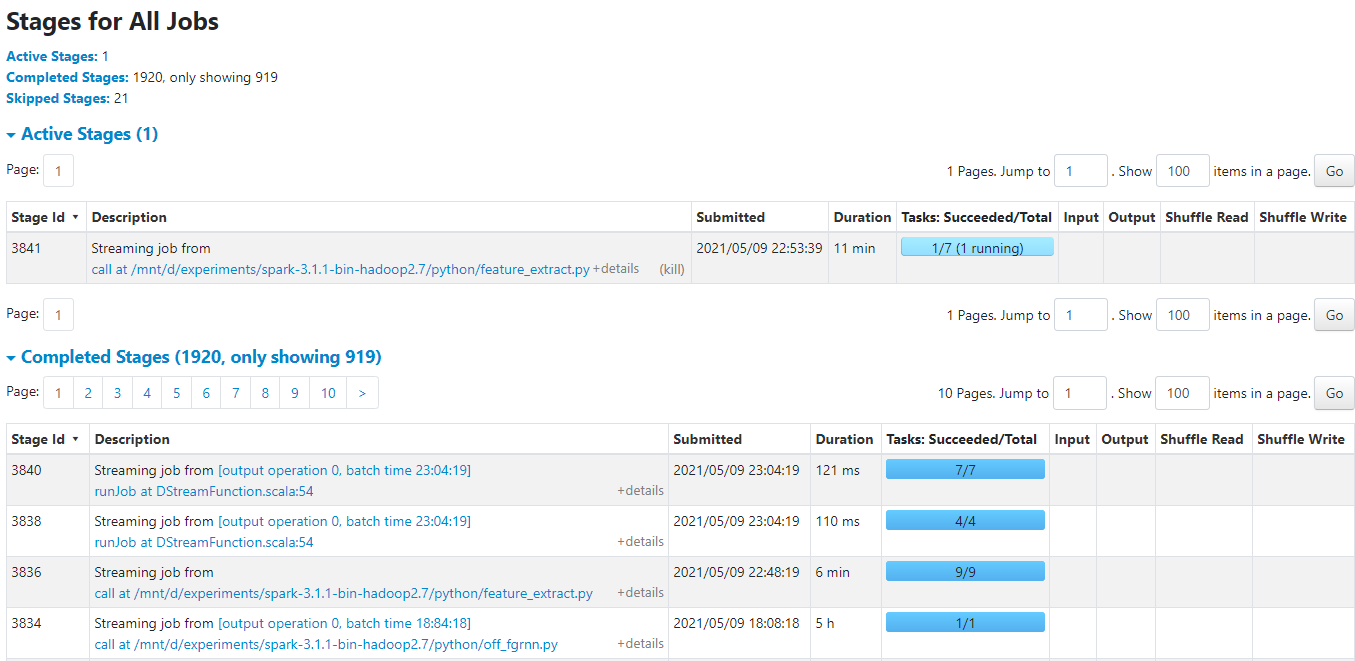
\includegraphics[width=1\linewidth]{spark-job-ui.png}
  \caption{Spark Web UI}
  \label{fig:spark-job}
\end{figure}

% 本节使用了第3章中CAMPUS数据集的第二段持续时长为18小时的数据作为系统的输入,经过测试,我们发现平均延迟3分钟即可将每个数据包的特征提取到相应的TCP/UDP流中,得到流的特征信息后,实时检测模块可以在1秒内输出异常类型。这得益于离线模型的定期更新。此外,我们还分析了该模型的失效时间,每次更新完一次模型的参数,可以看到随着时间的增长,模型效果越来越差,在5小时后准确率会低于60\%。
\section{系统运行结果}
我们在本系统中持续导入了约200小时的流量数据以验证该系统的有效性。系统共对15,998,551,646个packet进行分析,根据时间戳依次读取每个报文信息,提取特征,最终以5分钟为粒度汇报异常信息,累计汇报异常packet数量为3521687个,与此同时,SOC平台汇报异常packet总数为5496239个,总占比为64.07\%,具体的每类异常数量如图\ref{fig:每类异常数量对比}所示,其中远控木马、网络蠕虫、流氓推广、代码执行等类别的检出率偏低。我们将汇报结果与SOC平台中的告警信息进行对比,绘制了检测到的异常数量随时间变化图\ref{fig:异常数量}和异常准召随时间变化图\ref{fig:异常准召},图中横坐标为时间轴,从2021-03-19 13:30开始,到2021-3-20 19:30为止,以5分钟为一个刻度,从图中可以看出:
\begin{enumerate}
  \item 异常数量分布不均匀,异常数量会出现瞬间增多的现象,结合图4.14的CDF图可以看出,91\%的时间内异常数量在3000以内,1\%的时间内异常数量在28000以上。
  \item 以SOC平台作为groudtruth,本系统大部分时刻能够有效检测出85\%以上的异常,但是部分时刻召回率极低,仅有10\%左右,例如图中25、127、225三个时刻点,分别对应2021-03-19 15:20、2021-03-20 00:05和2021-03-20 08:15:00。以2021-03-19 15:20为例进一步分析,我们发现此时88\%的异常类型为远控木马,如图4.15所示,而本系统几乎未能检测出远控木马这类异常。远控木马具有持续性长,欺骗性强等特点,从流量特征来看,其与正常流量十分相似,可能会有长期的定时心跳包,仅凭这一点特征本系统难以检测此类型的异常。
  \item 对于长尺度时间而言,该系统在检测部分类别的异常时漏报率偏高,但是由于这部分异常本身占比不高,并且该系统的误报率较低,因此检测结果依然有一定参考价值。
\end{enumerate}

更具体地,我们选取了三个时刻点的数据进行进一步分析,如图4.15-4.17所示,当召回率极低时,往往是由于远控木马等难以检测的异常类别占比较高;而异常数量突增时,如果其组成成分多为拒绝服务、端口扫描等,系统的检测结果甚至会高于平均值。并且大部分时刻系统表现良好,能够有效检测出主要异常,且准确率较高。

% ,异常的分布很不均匀,80\%的时间内异常数量在300以内,1\%的时间异常数量在4000以上。异常峰值为2021-03-19 16:35:00 82283
% 2021-03-19 20:05:00 56424
% 2021-03-20 00:10:00 48579
% 2021-03-20 05:35:00 90963 四个时间窗。系统检测到此时占比最多的异常是远控木马。

% 以SOC的告警信息作为baseline,大部分时刻的检测准确率为85\%以上,
% 我们对不同的时间切片下进行了分析,
\begin{figure}
  \centering
  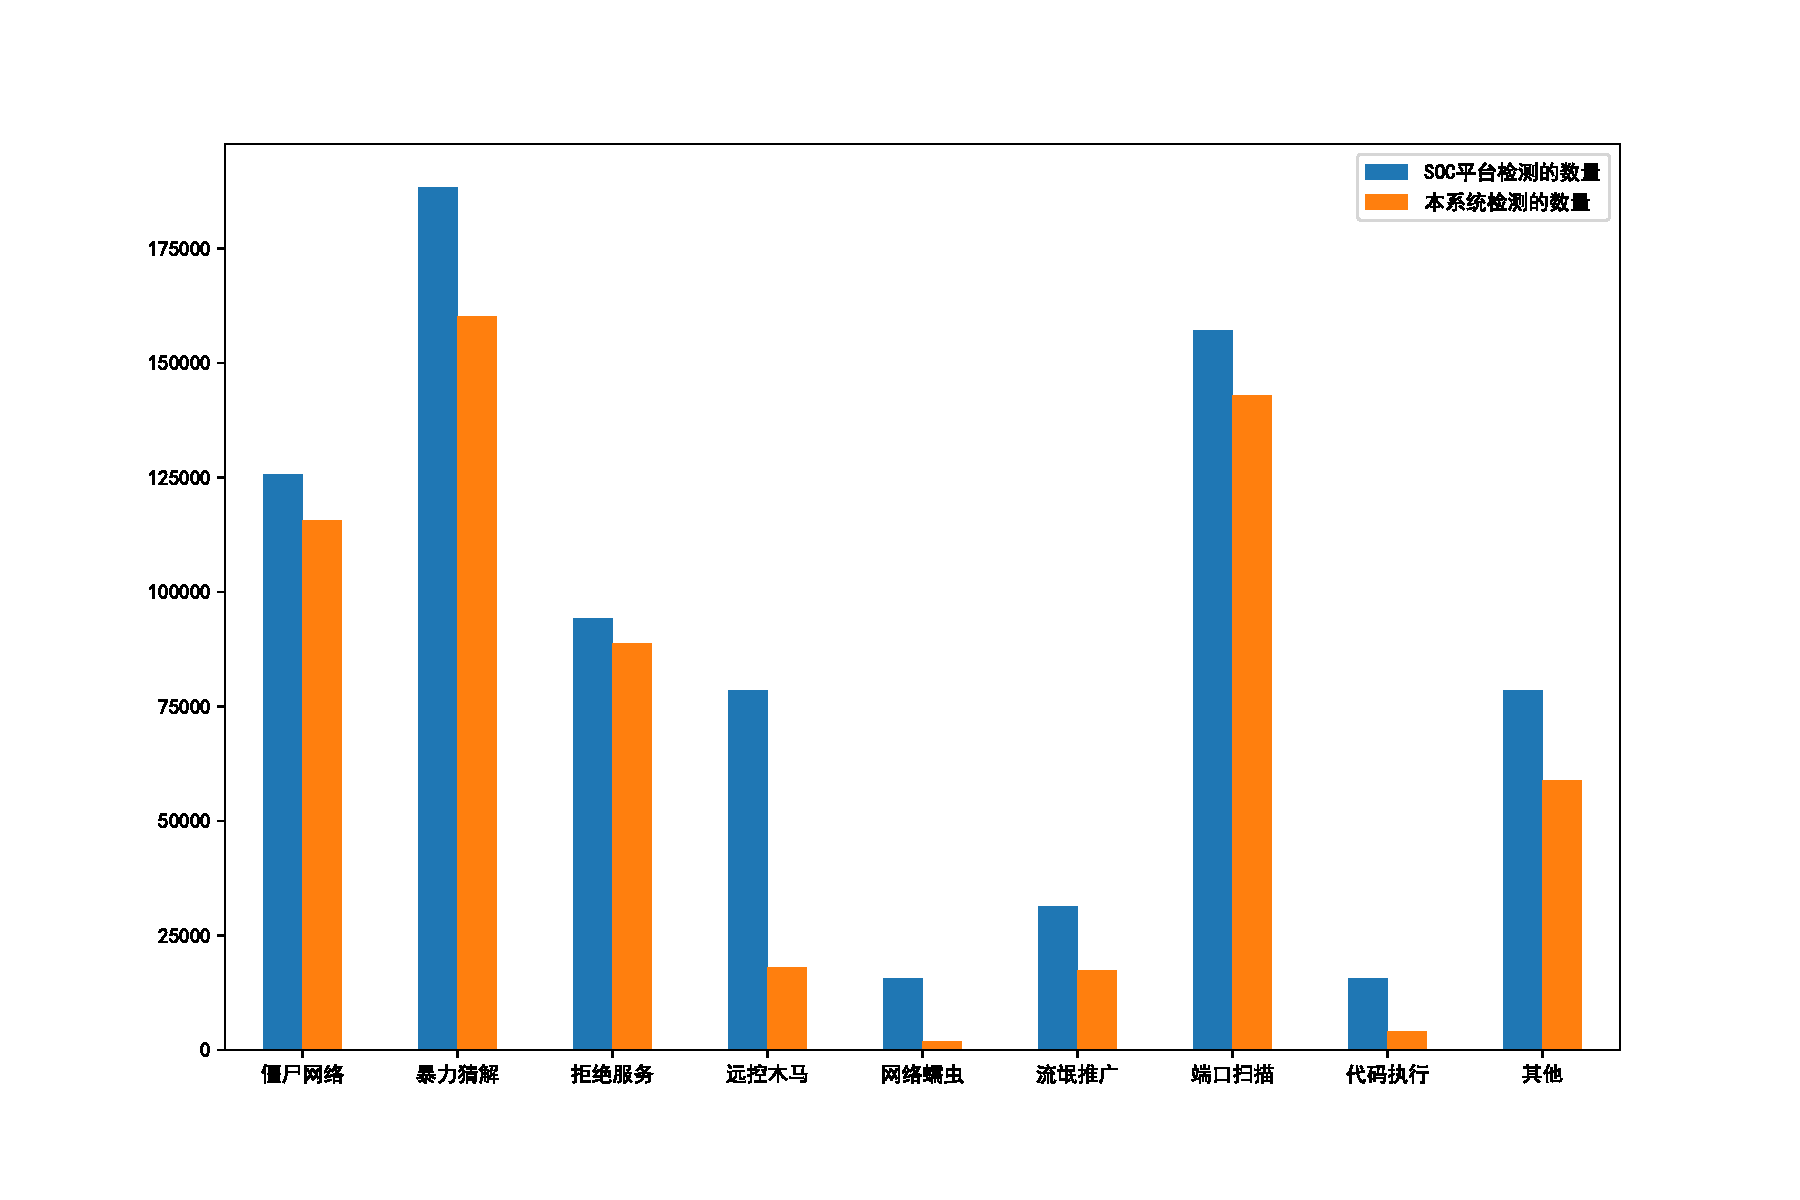
\includegraphics[width=1\linewidth]{检测到数量对比-30h.pdf}
  \caption{每类异常数量对比}
  \label{fig:每类异常数量对比}
\end{figure}


\begin{figure}
  \centering
  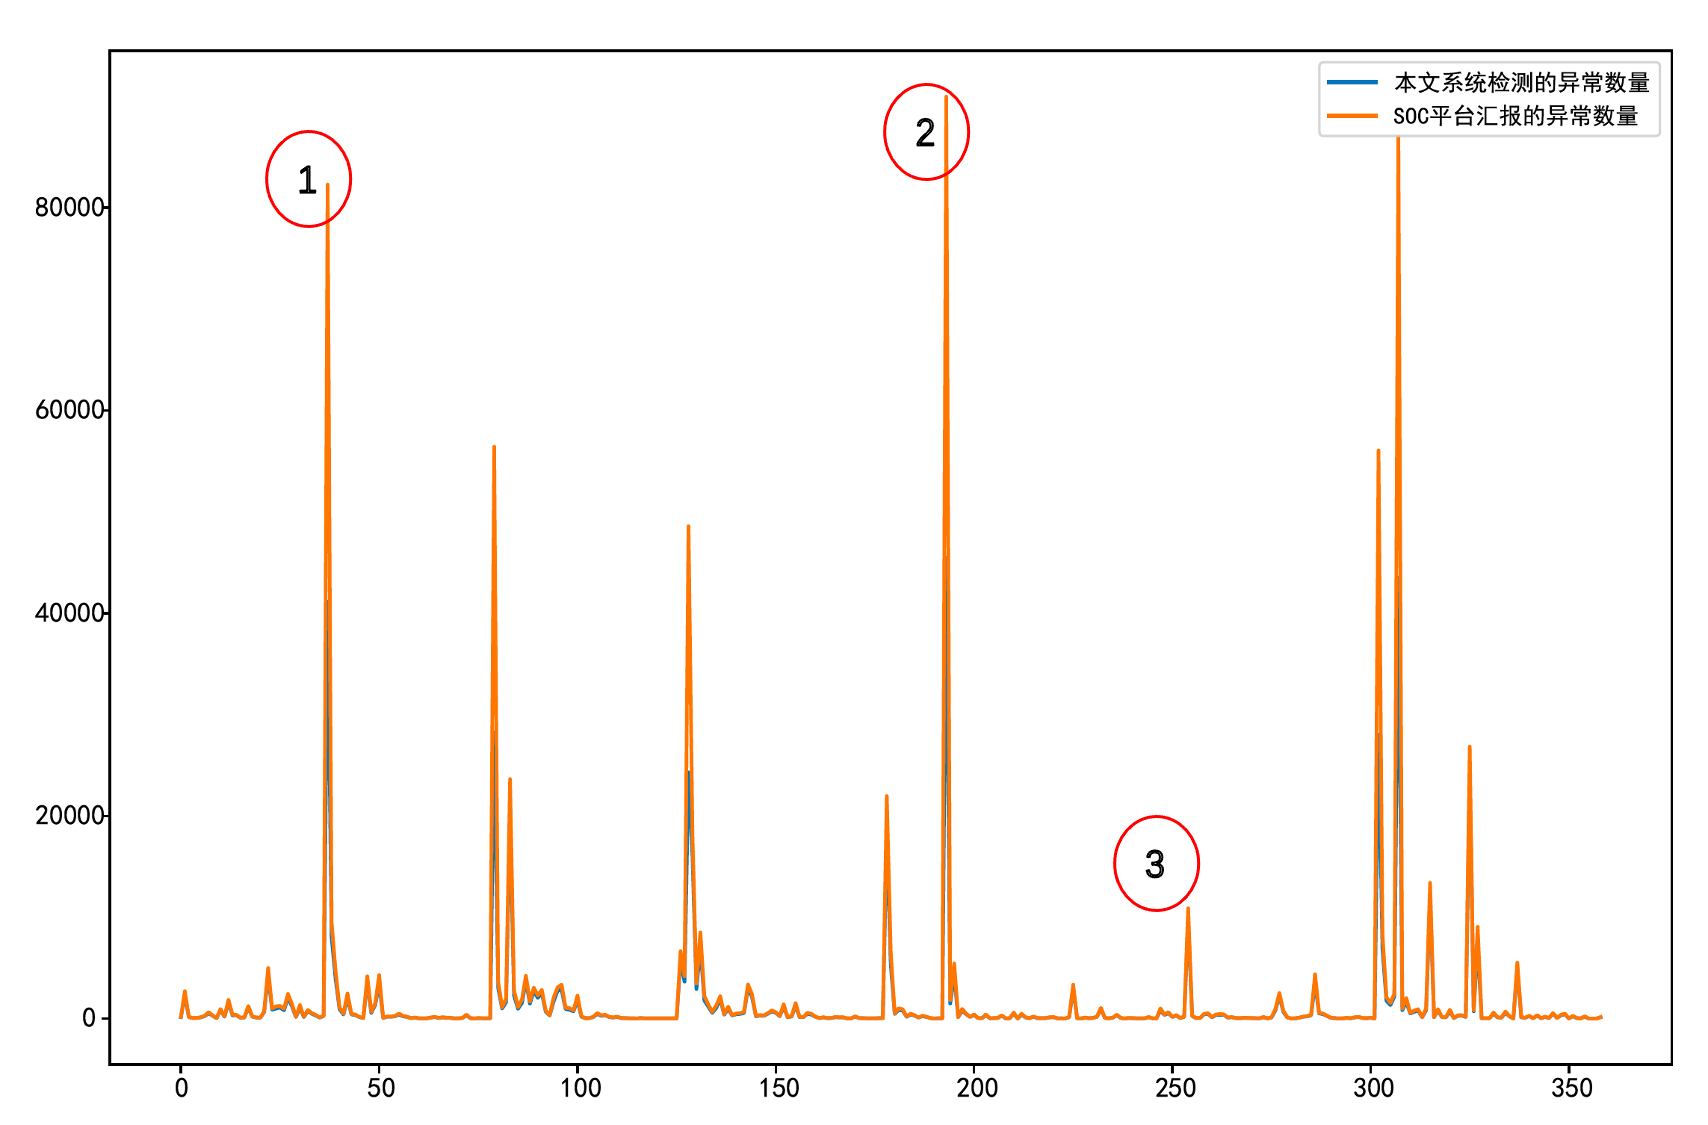
\includegraphics[width=1\linewidth]{异常数量随时间变化图.png}
  \caption{异常数量随时间变化图}
  \label{fig:异常数量}
\end{figure}

\begin{figure}
  \centering
  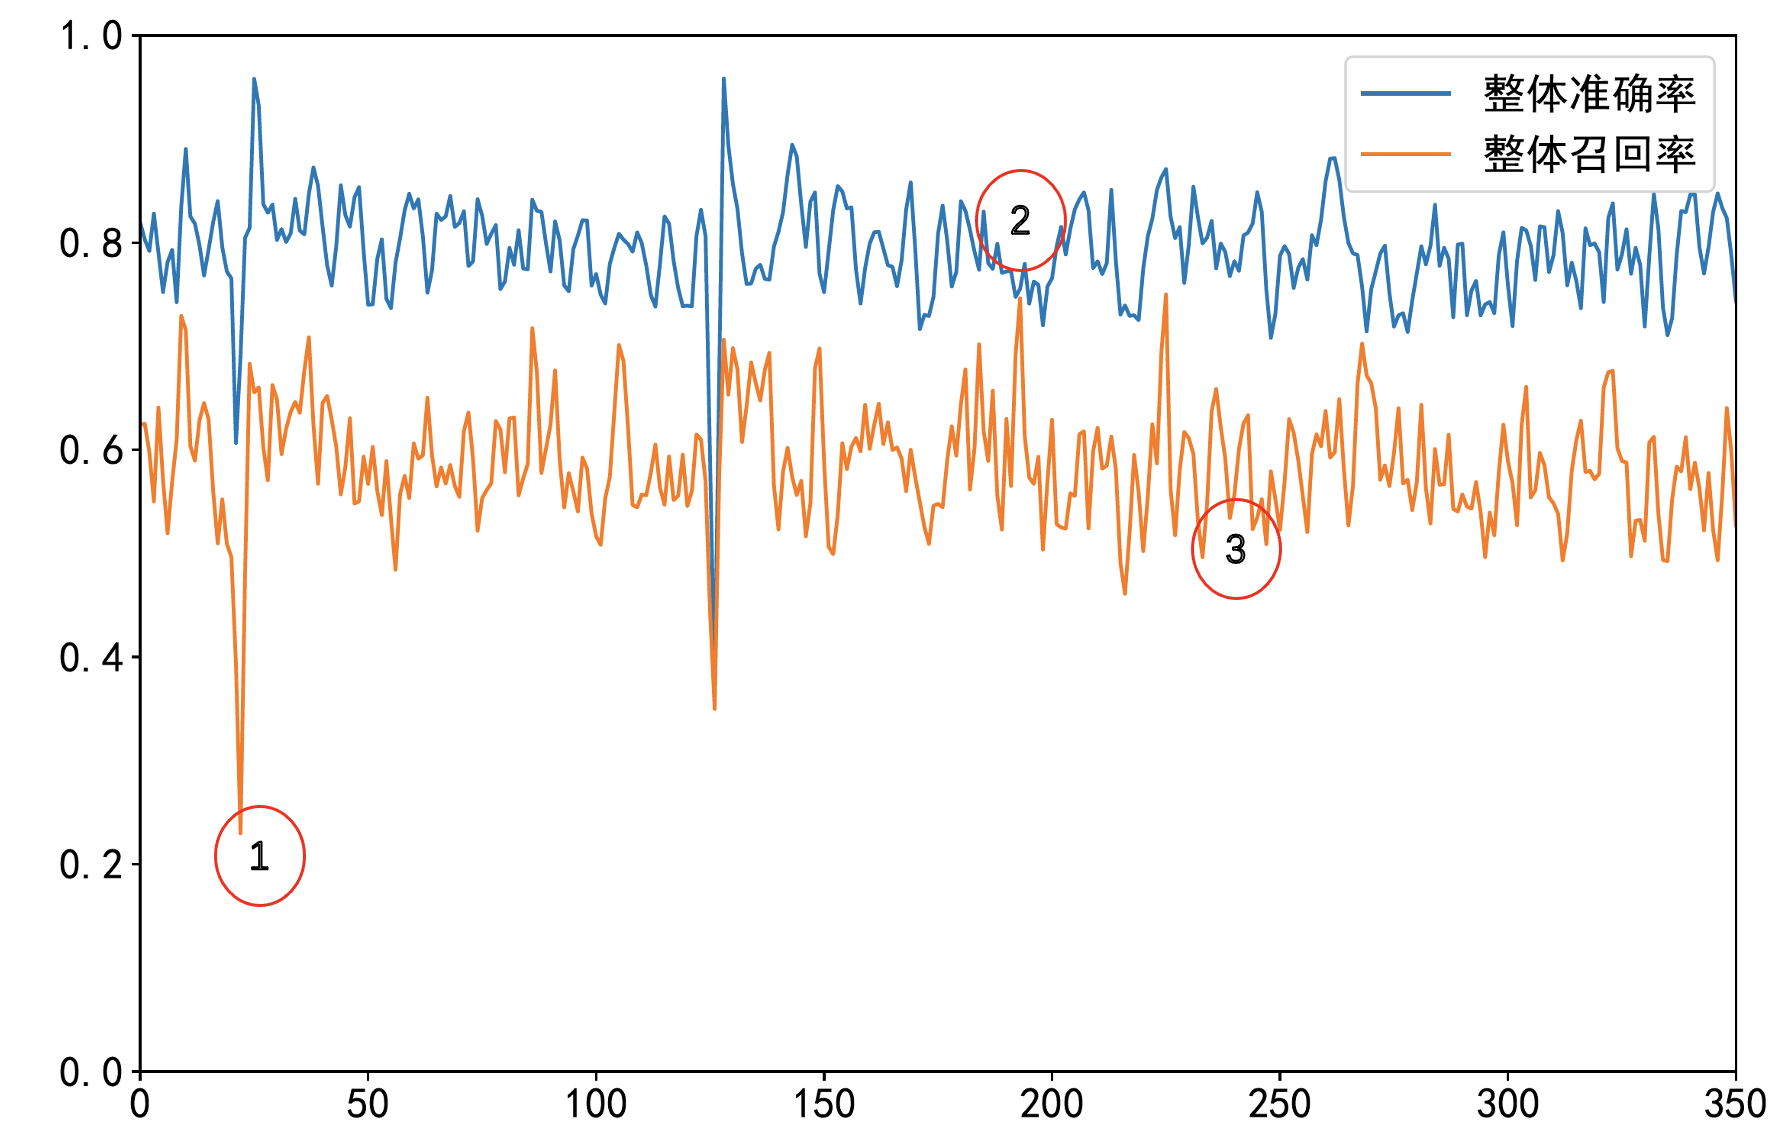
\includegraphics[width=1\linewidth]{异常准召随时间变化图.png}
  \caption{异常准召随时间变化图}
  \label{fig:异常准召}
\end{figure}

\begin{figure}[htbp]
  \centering
  \begin{minipage}[t]{0.48\textwidth}
  \centering
  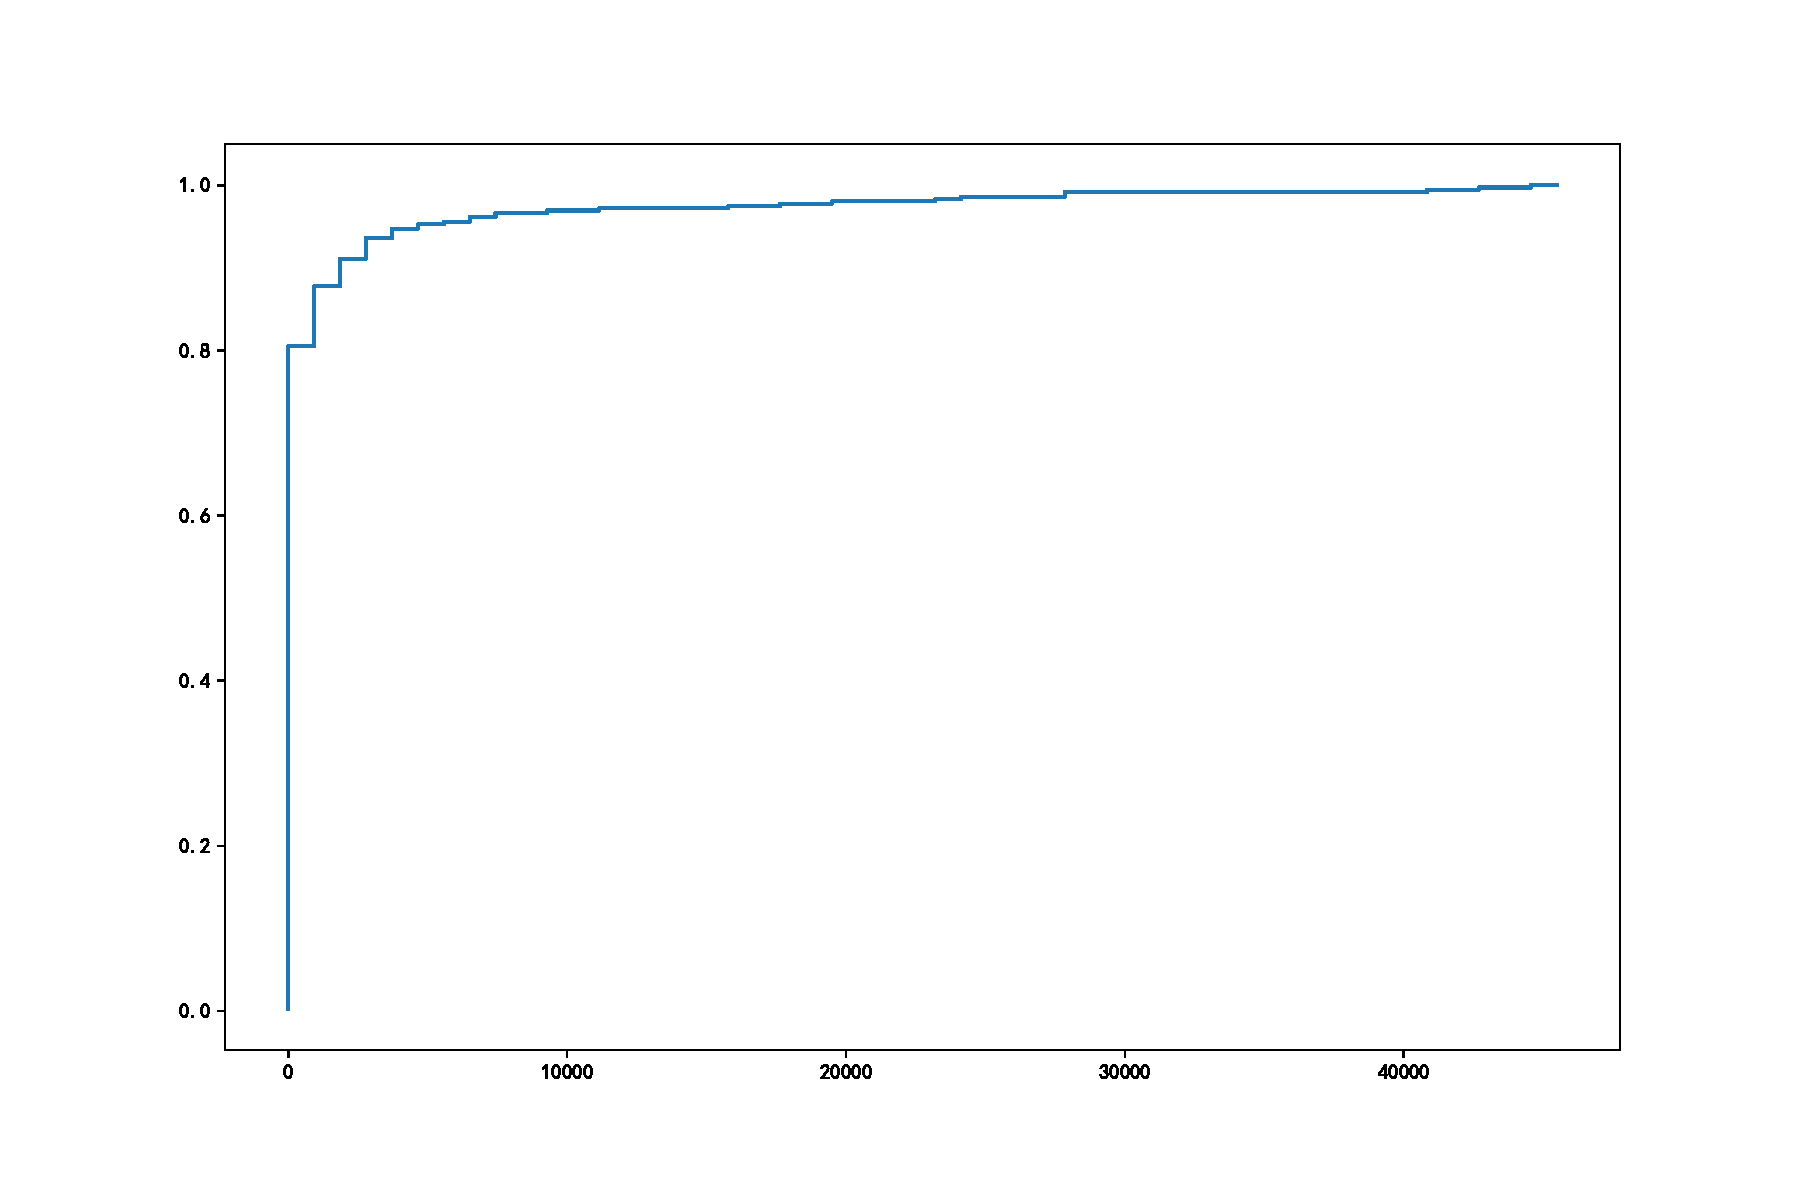
\includegraphics[width=1\linewidth]{异常数量cdf图.pdf}
  \caption{异常数量CDF图}
  \end{minipage}
  \begin{minipage}[t]{0.48\textwidth}
  \centering
  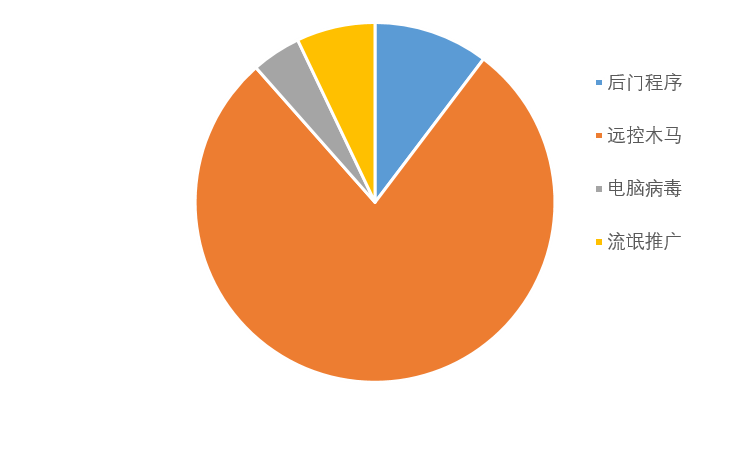
\includegraphics[width=1\linewidth]{15-20的异常分布.png}
  \caption{时刻1的异常分布}
  \end{minipage}
  \end{figure}

  \begin{figure}[htbp]
    \centering
    \begin{minipage}[t]{0.48\textwidth}
    \centering
    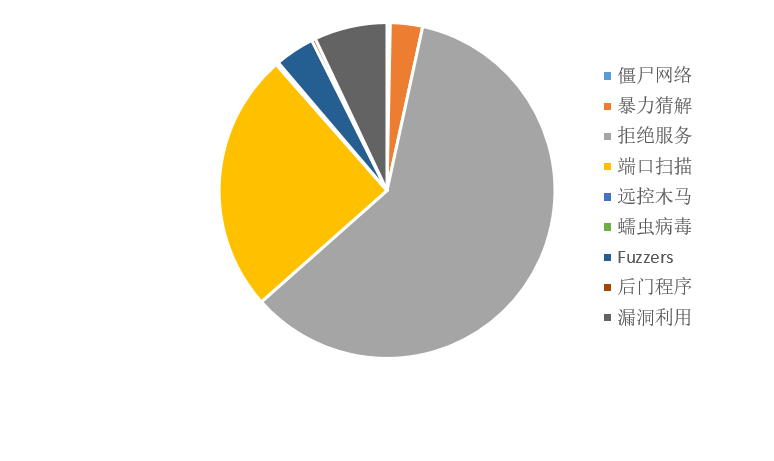
\includegraphics[width=1.2\linewidth]{时刻2的异常.png}
    \caption{时刻2的异常分布}
    \end{minipage}
    \begin{minipage}[t]{0.48\textwidth}
    \centering
    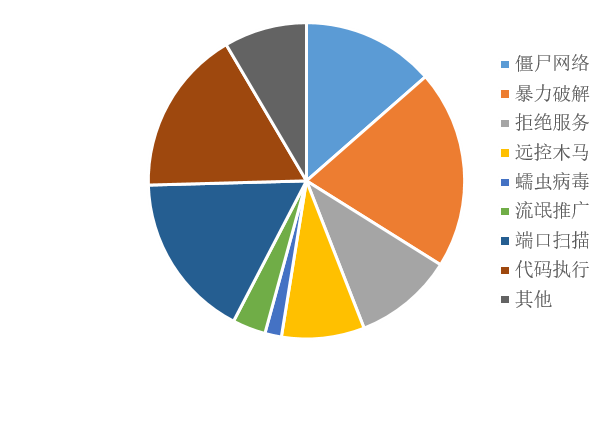
\includegraphics[width=1\linewidth]{时刻3的异常.png}
    \caption{时刻3的异常分布}
    \end{minipage}
    \end{figure}

% \begin{figure}
%   \centering
%   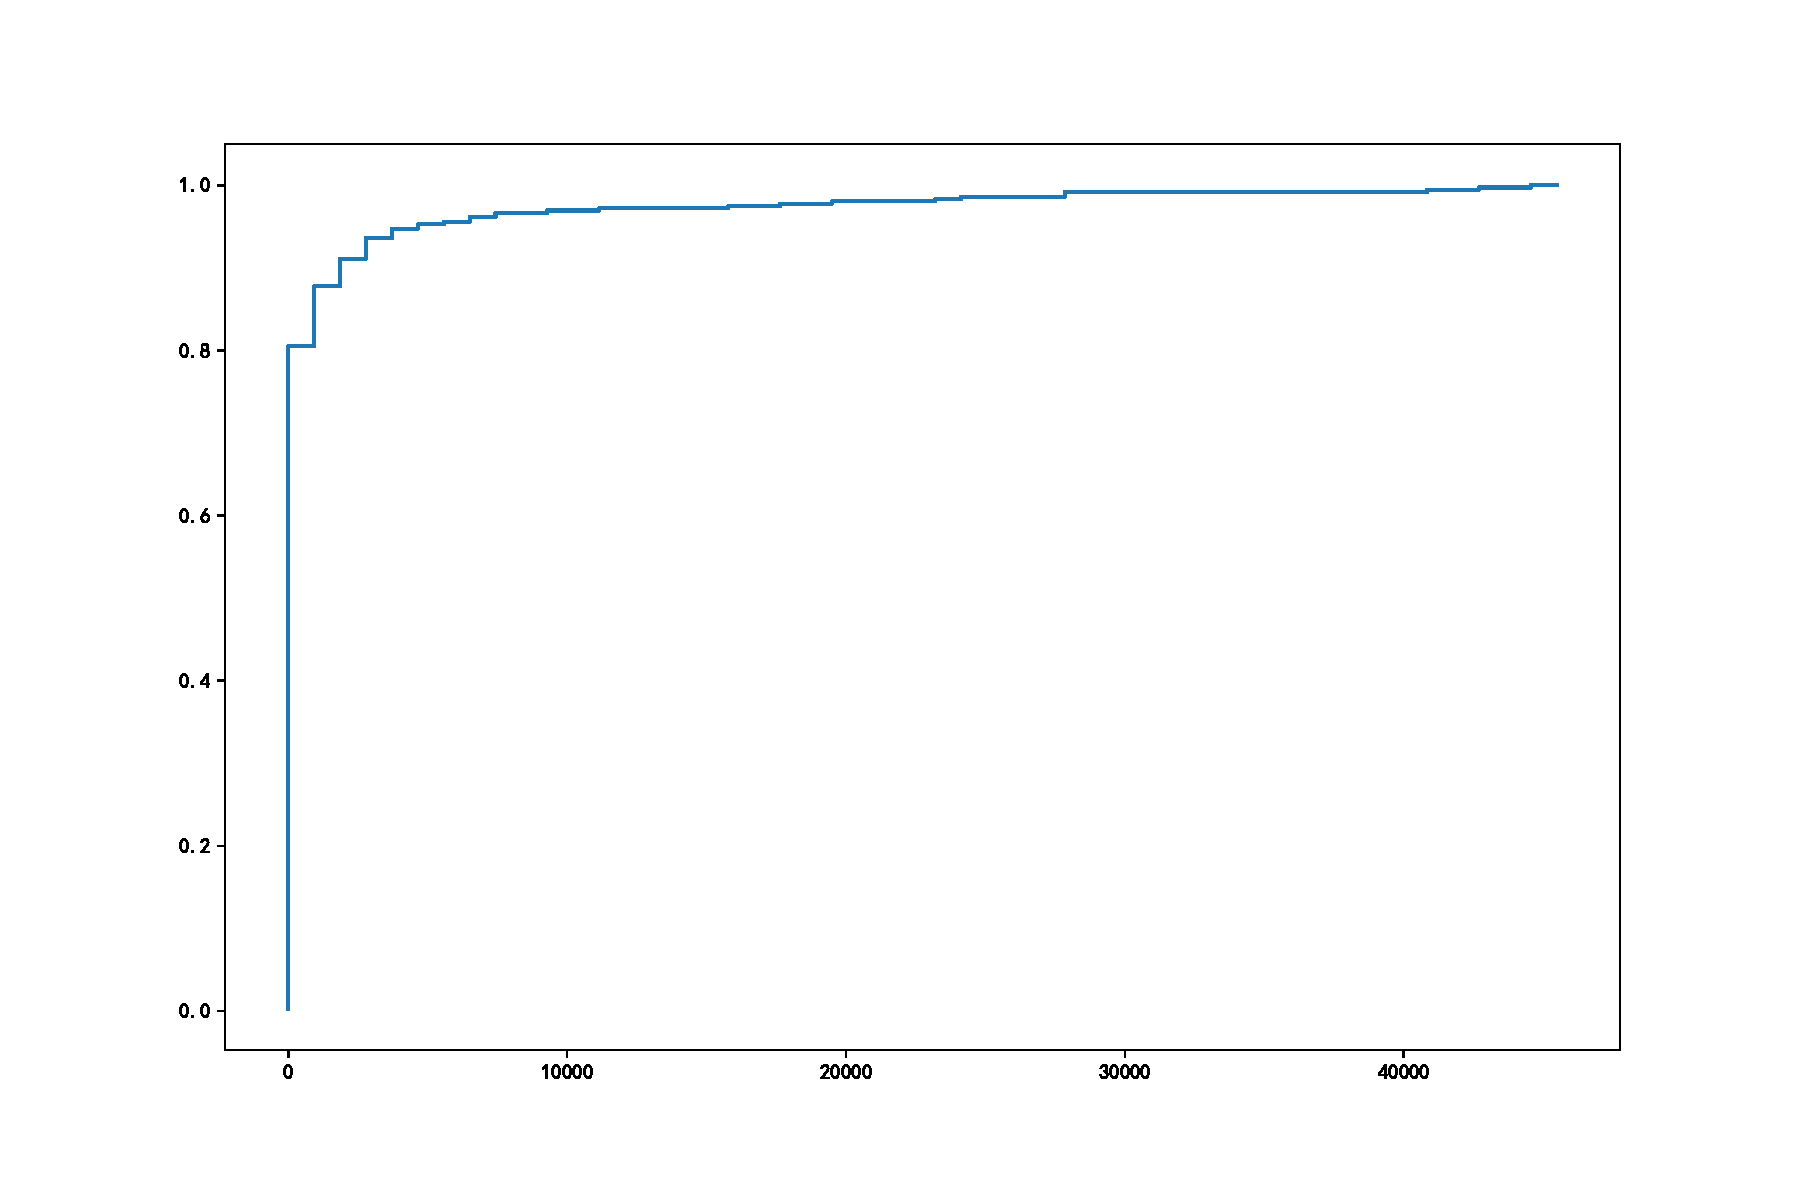
\includegraphics[width=1\linewidth]{异常数量cdf图.pdf}
%   \caption{异常数量CDF图}
%   \label{fig:异常数量CDF图}
% \end{figure}
% 僵尸网络的流量行为具有较强的规律性、周期性,暴力猜解的报文间隔很短,


\section{本章小结}
这一章设计并实现了一个流量异常检测系统,首先分别分模块对其进行了介绍,然后介绍了搭建系统的参数和流程,并且对系统运行结果进行了分析。
% 最后,对系统的部分运行结果进行了分析,并且介绍了系统在检测PortScan时的具体应用。

\chapter{异常检测系统在检测端口扫描中的应用}
在应用上述异常检测系统进行检测时,我们发现根据特征分析以及检测结果,该系统能够更有效地检测出DDoS、PortScan等异常。

本文发现在校园网vlan-pool架构下,出现大量PortScan时,由于外部主机试图访问内网不存在的主机,会在子网内部引发ARP报文,导致时延增高。PortScan本身是个安全问题,但是由于vlan-pool对ARP报文的放大效应,引发了一定的性能问题。
发现该问题后,为了定量分析PortScan对无线网性能的具体影响,本文首先搭建了一个小型子网进行了模拟仿真的受控实验,然后在校园网范围内进行了被动测量。验证端口扫描会对性能产生影响后,我们采用了封禁ip和增加缓存两种策略,有效降低了系统时延。

\section{受控实验}
为了验证端口扫描引发的大量ARP对无线网性能的定量影响,本文设计了一组受控实验,该实验的架构图如\ref{fig:受控实验架构图}所示,包含1个AP和10台终端设备,每台设备有着不同的物理速率。其中4台终端通过有线网连接到AP,用于控制ARP报文的数量,6台终端通过无线网连接到AP,用于控制局域网的整体负载。本文通过iperf控制AP的负载,nmap控制扫描流量的数量。值得注意的是,该局域网是一个IEEE 802.11ac 网络,将其安装在一个近似无干扰的环境中。 AP 在 5G 上以 100 Mbps 的数据速率运行,功率为 80mW。 各终端的物理速率如表\ref{每台终端的物理速率}所示,物理速率是指空口物理层的传输速率,是终端与ap协商的值,不是固定值;该表给出了各个终端大部分时间所处的物理速率。

\begin{figure}
  \centering
  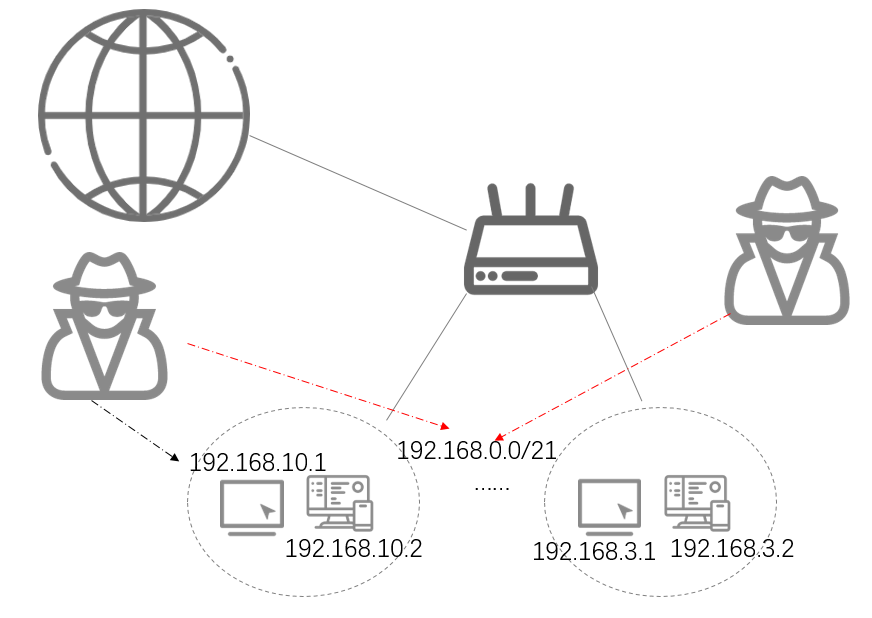
\includegraphics[width=0.6\linewidth]{port-scan-arch.PNG}
  \caption{受控实验架构图}
  \label{fig:受控实验架构图}
\end{figure}

\begin{table}[h] 
  \centering  %表格居中
  \caption{每台终端的物理速率}  %表格标题
  \label{每台终端的物理速率}
  \begin{tabular}{c|ccccc}
  \toprule  % 在表格最上方绘制横线
  devName&dev1&dev2&dev3&dev4&dev5\\
  \hline  %在第一行和第二行之间绘制横线
  Physical Rate&100&144&433&650&702\\
  \bottomrule
  \toprule % 在表格最下方绘制横线
  devName&dev6&dev7&dev8&dev9&dev10\\
  \hline  %在第一行和第二行之间绘制横线
  Physical Rate&780&780&866&866&866\\
  \bottomrule % 在表格最下方绘制横线
  \end{tabular}
  
  \end{table}

  本文将实验分成了九组,各组实验的参数设置如表\ref{每组实验的参数设置}所示。平均传输速率(Mbps)代表不同终端运行iperf产生的流量负载,而扫描范围代表不同终端运行nmap产生的扫描负载。 比如192.168.0.1/24代表扫描256个ip地址,192.168.0.1/21代表扫描2048个ip地址。 也就是说,case1-x 代表低流量负载场景,case2-x 代表中等负载,case3-x 代表高负载。 casex-1 代表无扫描环境,casex-2 代表中度扫描,casex-3 代表严重扫描。随着不同级别的流量负载和端口扫描负载,本文发现不同实验中子网具有不同的性能。 

\begin{table}[htb]
  \centering
  \caption{每组实验的参数设置}
  \label{每组实验的参数设置}
      \begin{tabular}{c|cc}
      \toprule  % 在表格最上方绘制横线
       &平均传输速率(Mbps)&扫描范围\\
      \hline  %在第一行和第二行之间绘制横线
      case1-0& 0 & 0\\
      \hline % 在表格最下方绘制横线
      case1-1& 0 & 16\\
      \hline  %在第一行和第二行之间绘制横线
      case1-2& 0 & 256\\
      \hline % 在表格最下方绘制横线
      case2-0& 87 & 0\\
      \hline % 在表格最下方绘制横线
      case2-1& 87 & 16\\
      \hline  %在第一行和第二行之间绘制横线
      case2-2& 87 & 256\\
      \hline % 在表格最下方绘制横线
      case3-0&470 & 0\\
      \hline % 在表格最下方绘制横线
      case3-1& 470 & 16\\
      \hline  %在第一行和第二行之间绘制横线
      case3-2& 470 & 256\\
      \bottomrule % 在表格最下方绘制横线
      \end{tabular}
\end{table}

% 在每组实验中,我们收集了单播报文数量、丢包率、端对端延迟

% 本文重点对比了高负载情况下无扫描和重扫描时 ARP 数量与延迟之间的关系。 在高负载情况下,如果子网充满了ARP包,延迟会比没有ARP包的情况增加100ms。

在每组实验中,我们收集了大量arp数量、单播报文数量、端对端延迟、丢包率、信道利用率等指标的数据。其中单播报文数量、信道利用率等指标是使用AirMagnet\cite{airmagnet}进行测量得到,端对端延迟是使用tcping测量得到,丢包率是从iperf输出日志得到。
不同组实验下信道利用率的比较如图~\ref{fig:信道利用率对比}所示,随着端口扫描流量的增加,信道利用率会增加10-20\%。图~\ref{fig:时延对比}是不同组别的实验中时延的对比情况,在网络处于中低负载时,尽管端口扫描增加,时延变化不大,仅在10-30ms之间波动。但是在高负载时,随着arp数量的增加,时延出现100ms以上的增加。这是因为arp数量的增加挤占了数据报文所需要的信道资源,导致数据报文丢包变多,从而时延增加。这点可以从图~\ref{fig:丢包率对比}中看出,在高负载情况下,端口扫描增加会出现丢包率增高的现象。
\begin{figure}
  \centering
  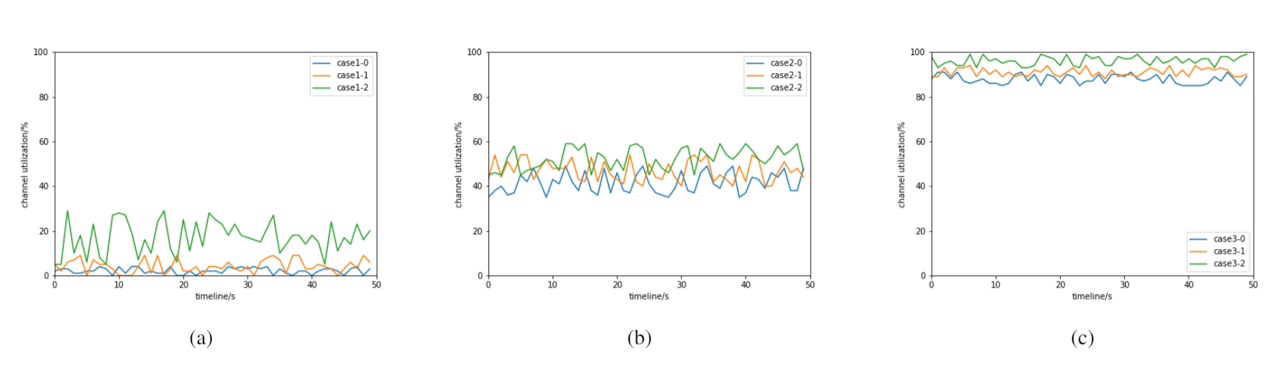
\includegraphics[width=1\linewidth]{long-cu.png}
  \caption{信道利用率对比}
  \label{fig:信道利用率对比}
\end{figure}

\begin{figure}
  \centering
  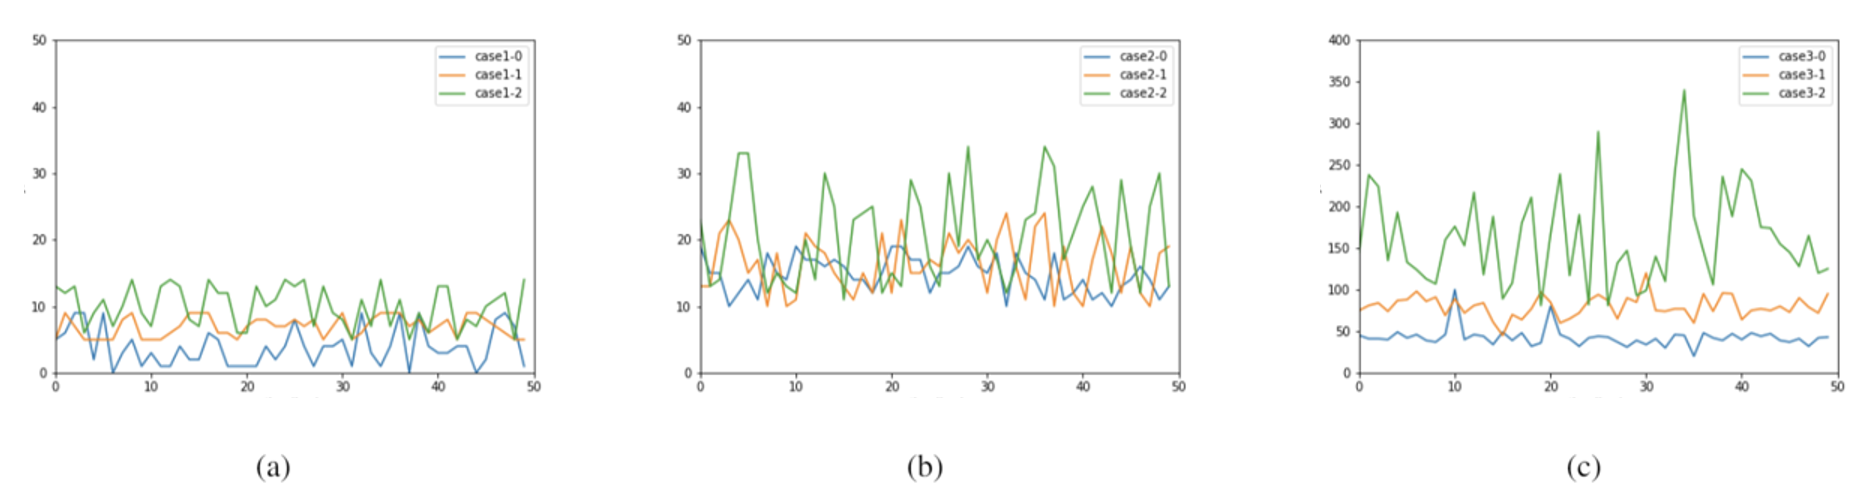
\includegraphics[width=1\linewidth]{long-timedelay.png}
  \caption{时延对比}
  \label{fig:时延对比}
\end{figure}

\begin{figure}
  \centering
  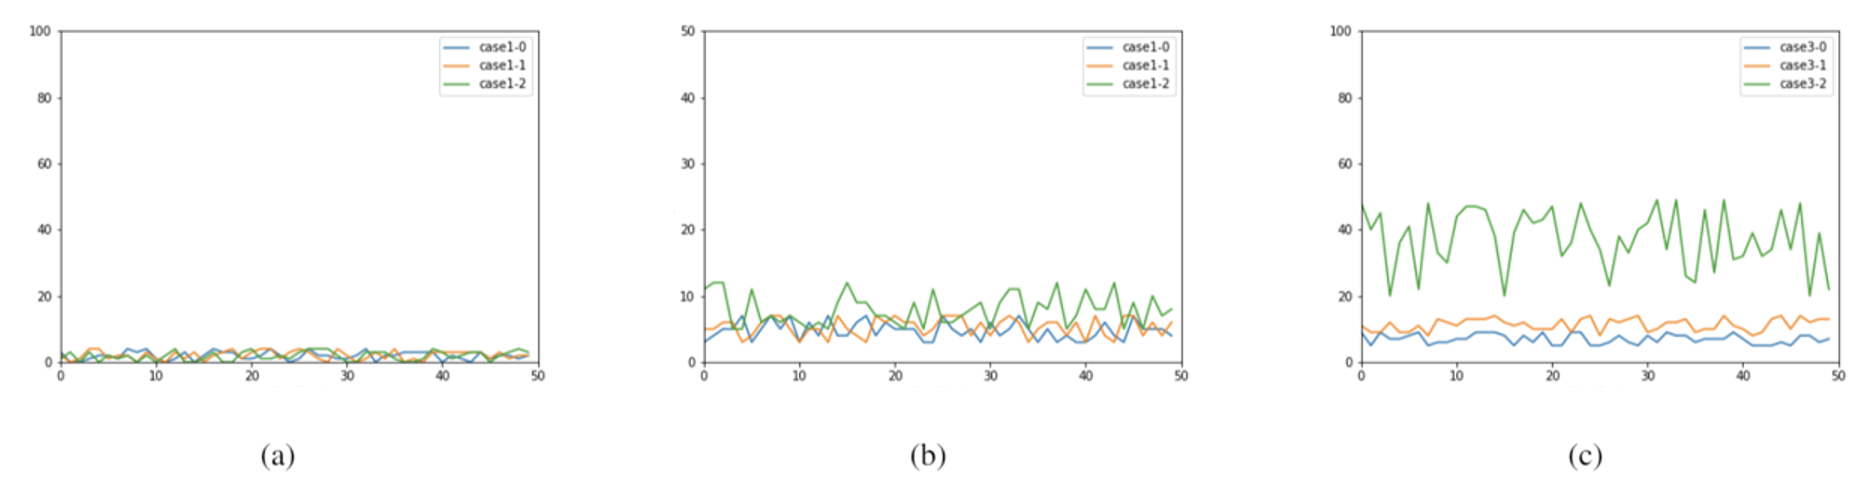
\includegraphics[width=1\linewidth]{long-drop.png}
  \caption{丢包率对比}
  \label{fig:丢包率对比}
\end{figure}
% 在本节中,我们分析这些数据以揭示 arp 数量与性能指标之间的定量关系。
% 不同情况下信道利用率的比较如图2所示。图 3 表示不同情况下的时间延迟。图4表示不同情况下的重传率。如图 2 所示,端口扫描流量导致通道利用率增加 10-20\%。中低负载时时延变化不大,而高负载时,大量端口扫描平均增加100ms以上。这是因为大量的端口扫描流量占用了更多的带宽,使得重传率增加,从而导致延迟增加。

% 我们进一步绘制图 5 以探索高负载情况下无扫描和重扫描时 arp 数与延迟之间的关系。在高负载情况下,如果子网中满是arp包,延迟会比没有arp包的情况增加100ms。

% \begin{figure}
%   \centering
%   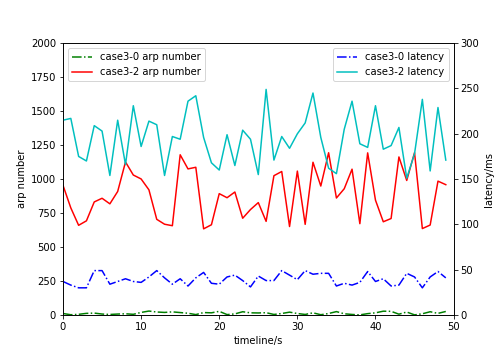
\includegraphics[width=0.6\linewidth]{case1-3-cmp.png}
%   \caption{case3实验结果对比}
%   \label{fig:case3实验结果对比}
% \end{figure}
\section{测量实验}
在进行受控实验后,我们在清华大学校园网中进行了大规模的测量,以验证端口扫描对无线网性能的影响。在本文中,本文收集了一周内的两种数据进行测量分析和评估,广播/单播包数据用于ARP分析,SNMP数据用于计算和衡量无线网的性能。广播/单播包数据由AirMagnet采集得到,SNMP数据通过SNMP轮询工具周期性抓取所需要的对象标识符得到。

% 重点写一下测量实验这部分 数据采集方案,

% 1.写一下数据有哪些类型,然后怎么得到的图表,然后分析一下图表中的结论。
% 2. 分析图表内容,over
% 3.特征增强实验的对比

简单网络管理协议(SNMP)是TCP/IP协议簇的一个应用层协议,被广泛应用于网络管理中\cite{perkins1997understanding}。针对一个给定的对象标识符(Object Identifier, OID),可以通过发起SNMP 请求以键值对的形式获取对象的值,用以监控设备或者网络的状态。

在本节中,我们主要采集以下几个OID:

\begin{itemize}
  \item 信道利用率(Channel Utilization):表示对于一个无线接入点来说,传输报文占用的时间比例。
  \item 传输的帧数(Transmitted Frames):表示在一个数据采集周期内,无线接入点成功传输的802.11 数据帧的数量。该OID定义为$Tran_{num}$。
  \item 重传的帧数(Retransmitted Frames):表示在一个数据采集周期内,由于无线链路层的丢包或者包错误(packet error)导致链路层重传的总帧数。该OID定义为$Retry_{num}$。
  \item 失败的帧数(Failed Frames):表示在一个数据采集周期内,在经历了一定次数的链路层重传尝试后最终传输失败的总帧数。该OID定义为$Failed_{num}$。
  \item 时延(Latency):终端侧的无线用户发送报文的平均延迟时间。该值为一段时间内的平均值。
\end{itemize}
利用上述部分OID我们可以计算出MAC层丢包率,即当无线MAC层发生丢包时,会重传相应的数据包,直到成功传输或重传次数达到预设阈值。其定义如下:
\begin{equation}
  % \sum_{i=1}^qd_{s-1,s}^i + d_{s,d} < \gamma\sum_{i=1}^qc_{s-1,s}^i
  {loss}_{mac} = \frac{{Retry}_{num} + {Fail}_{num}}{{Trans}_{num} + {Retry}_{num} + {Fail}_{num}}
\end{equation}

我们将采集到的数据按照arp数量进行对比,发现当网络中出现大规模端口扫描时,丢包率和时延都有增高。图~\ref{fig:丢包}和图~\ref{fig:时延}分别展示了某个AP下arp数量和时延、丢包率的关系。其中两图的横坐标为时间轴,每个坐标点代表5分钟,其中以78刻度作为分界线,左右两个区间内各自连续,纵坐标为双坐标轴,分别表示时延、丢包率、arp数量,均为5分钟内的平均值。从图中可以看出,arp报文数量增加到四倍时,丢包率从原来的3\%增加到20\%,而时延则提高到100ms以上。

\begin{figure}
  \centering
  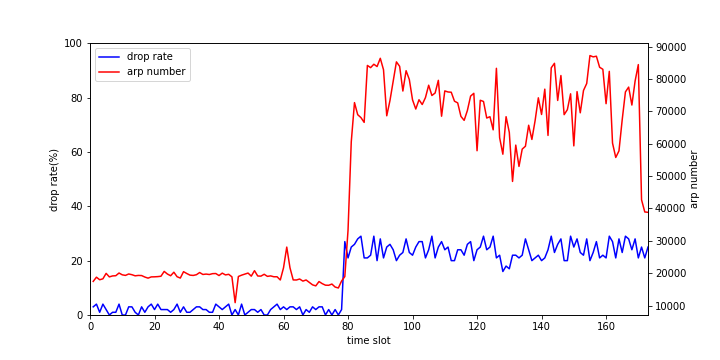
\includegraphics[width=1\linewidth]{drop_rate.png}
  \caption{arp数量和丢包率的关系}
  \label{fig:丢包}
\end{figure}

\begin{figure}
  \centering
  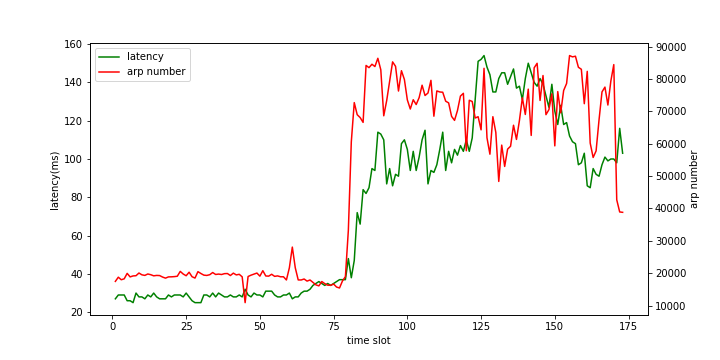
\includegraphics[width=1\linewidth]{latency_mea.png}
  \caption{arp数量和时延的关系}
  \label{fig:时延}
\end{figure}
\section{优化策略}
在以上基础上,我们采用了两种优化策略。
\begin{enumerate}
  \item 在出口网关处进行端口扫描ip的封禁,由第四章的异常检测系统提供端口扫描ip的列表,然后运维人员对这些ip地址进行封禁操作。
  \item 在AC中添加当前子网已分配ip地址的缓存,该缓存为关联在当前AP上的设备mac与对应ip地址的映射表。判断流程如图\ref{fig:优化策略}所示,每当AP收到一个报文,首先查看ip地址是否存在于映射表中,如果在则说明该ip已分配给某台设备,直接转发该报文,不会产生arp;如果ip地址不在映射表中,则需要判断表中是否存在未分配ip地址的设备mac,如果存在,需要下发相应的arp报文,如果不存在,则直接将报文丢弃。因为当出现漫游设备时,映射表中该设备mac可能没有对应的ip地址,即此时$n$个设备关联在AP上,只有$m$($m<n$)个ip地址已分配。
  % 当设备上线认证时,将其ip地址添加到缓存中,设备下线或者超时时,从缓存中删除该ip地址。
\end{enumerate}
\begin{figure}
  \centering
  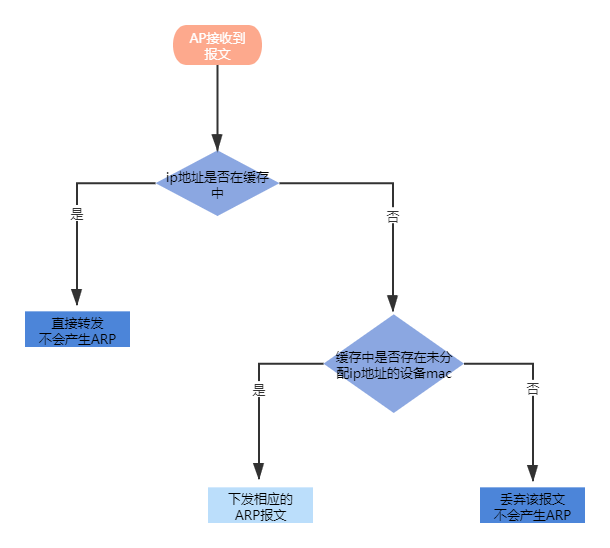
\includegraphics[width=1\linewidth]{优化策略.png}
  \caption{增加缓存的优化策略}
  \label{fig:优化策略}
\end{figure}
经过仿真验证,这两种策略均能有效降低arp数量,并且在外部扫描依然存在的情况下,子网平均时延由150ms下降到50ms左右。
% 一是在出口网关处进行端口扫描ip的封禁,由第四章的异常检测系统提供端口扫描ip的列表,然后运维人员对这些ip地址进行封禁操作;二是在AC中添加当前子网已分配ip地址的缓存,当设备上线认证时,将其ip地址添加到缓存中,设备下线或者超时时,从缓存中删除该ip地址。经过仿真验证,这两种策略均能有效降低arp数量,并且在外部扫描依然存在的情况下,子网平均时延由150ms下降到50ms左右。

% 二是缓存机制,在AC中加入一个设备mac和已分配ip地址的映射表,当发生,逻辑框图如下,1.设备数和ip地址数一致,2.不一致,
% 每当AP收到一个报文,先去查看ip地址是否存在于映射表中,如果在则说明已分配给某个具体的设备,直接进行转发,如果不在则进一步判断标记位,标记位为1,直接丢弃,为0,依然要进行转发。在这个过程中,不会对扫描报文进行转发,大大降低arp数量。 当设备出现漫游时,n个设备关联在AP上,只有m个ip分配出去。

\section{本章小结}
通常端口扫描被视为一个安全问题,在前述章节中这类异常可以有效地被检测系统检测到,但是本章发现端口扫描会对无线网性能产生一定影响。当发生对子网中不存在的ip进行扫描时,由于vlan-pool架构中一个AP可以工作在多个vlan下,该AP会在所有vlan中发送该ip地址相关的ARP报文,产生ARP泛洪。本章通过受控实验和测量实验,验证了该现象,并且使用封禁ip和增加缓存策略,有效缓解了该问题。